\documentclass[ruledheader,noindentfirst,anapcustomindent,abntfigtabnum,tocpage=plain]{def_and_cls/abnt}
\usepackage{amsmath, amssymb, amsthm, verbatim, amsfonts, amstext}
%\usepackage[latin1]{inputenc}
\usepackage[brazilian]{babel}
\usepackage[utf8]{inputenc}
\usepackage[T1]{fontenc}
\usepackage{styles/dropping}
\usepackage{graphicx}
\usepackage[hang,small,bf]{caption}
\usepackage[abnt-etal-list=0,abnt-etal-text=it,abnt-and-type=&,abnt-emphasize=bf,abnt-full-initials=yes,alf,bibjustif]{styles/abntcite}
\usepackage{fancyhdr}
\usepackage{makeidx}
\usepackage[none]{hyphenat}
\usepackage{color}
\usepackage{subfig}
\usepackage{styles/algorithms}
\usepackage{algorithmic}
\usepackage{mdwlist}
\usepackage{bm}
\usepackage[titletoc,title]{appendix}
\usepackage{ltxtable}
\usepackage{longtable}
\usepackage{supertabular}
\usepackage{indentfirst}
\usepackage{color}
\usepackage{icomma}

% \usepackage{biblatex} %Imports biblatex package
% \addbibresource{mybibliography.bib} %Import the bibliography file

\usepackage[
    backend=biber,
    style=alphabetic,
    sorting=ynt
]{biblatex}

\addbibresource{bib.bib} %Imports bibliography file

\usepackage[table,xcdraw]{xcolor}
\usepackage{pdfpages}

\usepackage{adjustbox}
\usepackage{tabularray}
\usepackage{xurl}

\sloppy


%
%Tradução do pacote Algorithm para portugues
%
\renewcommand{\algorithmicrequire}{\textbf{Entrada:}}
\renewcommand{\algorithmicensure}{\textbf{Saída:}}
\renewcommand{\algorithmicend}{\textbf{fim}}
\renewcommand{\algorithmicif}{\textbf{se}}
\renewcommand{\algorithmicthen}{\textbf{então}}
\renewcommand{\algorithmicelse}{\textbf{senão}}
\renewcommand{\algorithmicelsif}{\algorithmicelse \, \algorithmicif}
\renewcommand{\algorithmicendif}{\algorithmicend \, \algorithmicif}
\renewcommand{\algorithmicfor}{\textbf{para}}
\renewcommand{\algorithmicforall}{\textbf{para todo}}
\renewcommand{\algorithmicdo}{\textbf{fazer}}
\renewcommand{\algorithmicendfor}{\algorithmicend \, \algorithmicfor}
\renewcommand{\algorithmicwhile}{\textbf{enquanto}}
\renewcommand{\algorithmicendwhile}{\algorithmicend \, \algorithmicwhile}
\renewcommand{\algorithmicloop}{\textbf{laço}}
\renewcommand{\algorithmicendloop}{\algorithmicend \, \algorithmicloop}
\renewcommand{\algorithmicrepeat}{\textbf{repetir}}
\renewcommand{\algorithmicuntil}{\textbf{até}}
\renewcommand{\algorithmiccomment}[1]{\{#1\}}
\renewcommand{\listalgorithmname}{Lista de Algoritmos}
\floatname{algorithm}{Algoritmo}
%%%%%%%%%%%%%%%%%%%%%%%%%%%%%%%%%%%%%%%%%%%%%%%%%%%%%%%%%%%%%%%%%%%%%%%%%%%%%%%%%%%

\makeindex

%%%% O arquivo modelosCAP.tex possui as definições para ciação do estilo de capítulo (fonte de título, barras horizontais, etc.)
% ele não gera texto de saída, é um arquivo de configuração somente
%
\input{0.1-modelosCAP}
%%%%%%%%%%%%%%%%%%%%%%%%%%%%%%%%%%%%%%%%%%%%%%%FIM DO PREAMBULO%%%%%%%%%%%%%%%%%%%%%%%%%%%%%%%%%%%%%%%%%%%%%%%%%%%%%%%%%%%%%%%%%%


\begin{document}

%%%%% IMPORTANTE: ALTERA O TEXTO ENTRE ARIAL E TIMES NEW ROMAN (ALTERNAR OS COMENTÁRIOS)
%
%%%%%%%%%%%%%%%%%%%%%PARA UTILIZAR ARIAL%%%%%%%%%%%%%%%%%%%%%%%
%
\fontfamily{phv}                    %fonte Arial
\renewcommand{\rmdefault}{phv}      %
%
%%%%%%%%%%%%%%%%%%%%%PARA UTILIZAR TIMES%%%%%%%%%%%%%%%%%%%%%%%
%
%\fontfamily{ptm}               %fonte Times
%\renewcommand{\rmdefault}{ptm} %
%
%%%%%%%%%%%%%%%%%%%%%%%%%%%%%%%%%%%%%%%%%%%%%%%%%%%%%%%%%%%%%%%

%%%%%%%%%%%%%Arquivos .tex com os elementos pré-textuais
%
\thispagestyle{empty}

\vfill
 \begin{center}
    {\large\bfseries ESCOLA POLITÉCNICA DA USP} \\
    \vspace*{1in}
    \begin{figure}[h]
     \centering
            \includegraphics[width=10cm]{figures/Logo_Poli.jpg}\\
     \end{figure}
    \vspace*{1in}
    \large\bfseries MONOGRAFIA DE SISTEMAS EMBARCADOS\\
    
    ESTABILIZADOR GIMBAL DE BAIXO CUSTO\\
    
    \vspace{1.5cm}
    ANA CLARA FORCELLI - 10773631\\
    ARTHUR PIRES DA FONSECA - 10773096\\
    BRENO LOSCHER ROCHA - 9784439\\
    \vfill
    \large\bfseries{ SÃO PAULO \\ 2022}
\end{center}

\normalsize
\begin{titlepage}
\vfill
\begin{center}
    \vspace{2cm}
    {\Large \textsc{MONOGRAFIA DE SISTEMAS EMBARCADOS\\
    ESTABILIZADOR DE CÂMERA DE BAIXO CUSTO}\\}
    \vspace{1cm}
    \hspace{.45\linewidth}
    \begin{minipage}{.50\linewidth}

            Um estabilizador 'gimbal' open-hardware e open-source utilizando materiais acessíveis

            \vspace{0.5 cm}

            Orientadores: \\
            Prof. Dr. Bruno C. Albertini\\
            Prof. Dr. Moacyr Martucci Junior\\
            Eng. Olimpio Rodrigues
    
    \end{minipage}

    \vspace{2cm}
    \vfill
    {\large SÃO PAULO\\ 2022}
\end{center}

\end{titlepage}
\includepdf[pages=1,scale=1,pagecommand={},linktodoc=true]{ficha.pdf}
\include{3-folhadeaprovacao}
\chapter*{Dedicatória}

\noindent Dedico este trabalho à Hihi e aos meus avós por terem cuidado de mim, ao meu irmão (o Di), e aos meus pais, Alfredo e Márcia.

\noindent Dedico este trabalho ao meu amigo Mario Granziera e aos meus pais, Júlia e Antônio.
\chapter*{Agradecimentos}

\noindent Agradecimentos texto.\\

Agradecemos ao Guilherme Migliati https://www.linkedin.com/in/guimigli?utm_source=share&utm_campaign=share_via&utm_content=profile&utm_medium=android_app foram essenciais para superar obstáculos no desenvolvimento do aplicativo, oferecendo suporte técnico, que permitiu a compilação dele.

\\

Além disso, a contribuição significativa do Dr.-Ing. Philippe Jardin https://www.linkedin.com/in/dr-ing-philippe-jardin-964733a3?utm_source=share&utm_campaign=share_via&utm_content=profile&utm_medium=android_app , que disponibilizou o simulador de OBD quando o Arthur ainda estava na Alemanha, ampliou consideravelmente as capacidades de teste do sistema. 

\chapter*{Epígrafe}

\noindent Epígrafe texto.\\
\pagestyle{plain}%%%%% Utilizar ESTILO PLAIN AQUI%%%%%%%
\chapter*{Resumo}

\noindent Visando criar uma plataforma complementar ao motorista e seu carro, este trabalho usará sensores diversos ao redor de um automóvel para analisar o perfil de condução dessa pessoa.\\
A coleta será feita por uma porta OBD-II, presente em todos os veículos fabricados a partir de 2010 no Brasil.\\ 
Os dados, por sua vez, serão passados para a nuvem, para análise de perfil de cada condutor.\\ 
Cada condutor poderá consultar seus dados pessoais por um sistema com autenticação, exercitando, neste trabalho, a implementação da segurança, um aspecto fundamental para a proteção de dados.

\chapter*{Abstract}


\noindent Aiming to create a complementary platform to the driver and his car, this work will use various sensors around a car and from a smartphone, for example, to develop a data capturing platform. \\
The collection will be done through an OBD-II port, available in all vehicles manufactured since 2010 in Brazil. \\
The data, in turn, will be transferred to the cloud for profile analysis of each conductor. \\
Each driver will be able to consult their personal data through a system with authentication, which is an exercise of implementation of security, an aspect fundamental to data protection.

%%%Comandos para criação automática das listas
%
\tableofcontents
\listoffigures
\listoftables

%%%Comandos para criar outras listas não suportadas pelo pacote ABNTex%%%
%
% \pretextualchapter{Lista de Símbolos}
% \input{12-nomenclatura}
% \newpage

\pretextualchapter{Lista de Abreviações}
\begin{basedescript}{\desclabelstyle{\pushlabel}\desclabelwidth{6em}}
\item[{IoT}] \textit{Internet of Things}
\item[{OBD-II}] \textit{On-board diagnostics}
\item[{MVP}] \textit{Minimum Viable Product}
\item[{IDE}] \textit{Integrated Development Environment}
\item[{JSON}] \textit{Java Script Object Notation}
\item[{API}] \textit{Application Programming Interface}
% \item[{fda}] Função de distribuição acumulada%
% \item[{EMQ}] Erro médio quadrático%
\end{basedescript}
\newpage
%%%%%%%%%%%%%%%%%%%%%%%%%%%%%%%%%%%%%%%%%%%%%%%%%%%%%%%%%%%%%%%%%%%%

%Capítulos passam a ter páginas numeradas
%
\pagestyle{fancy}

%resseta os contadores de capítulo e seção
%
\renewcommand{\chaptermark}[1]{\markboth{#1}{}}
\renewcommand{\sectionmark}[1]{\markright{\thesection\ #1}}

%%%%%%%%%%%%%%NÃO LEMBRO O QUE FAZ, APARENTEMENTE NADA, TESTAR DEPOIS
%\fancyhf{}%
%\fancyhead[RO,LE]{\large\slshape\thepage}%
%\fancyhead[CE]{\large\slshape\leftmark}%
%\fancyhead[CO]{\large\slshape\rightmark}%


%%% Outros arquivos .tex. É acoselhável utilizar vários arquivos, pelo menos um por capítulo
\chapter{Introdução}\label{CAP:introducao}

Este documento detalha a concepção e implementação de um sistema dedicado à aquisição e análise de dados relacionados à condução de um motorista.

A abordagem central consiste na extração de informações provenientes de sensores já presentes em veículos contemporâneos, acessando a porta OBD-II, que adota um padrão internacional para o diagnóstico de parâmetros internos de um automóvel\textsuperscript{[2]}.

Adicionalmente, são coletadas informações fornecidas por um dispositivo móvel, incluindo dados de geolocalização e acelerômetros, e essas informações são centralizadas em uma base de dados hospedada na AWS. 

Esta arquitetura permite uma análise posterior aprofundada desses dados, promovendo \textit{insights} valiosos sobre os padrões e comportamentos de direção.

\section{Motivação}

Buscando traçar o perfil de condução de um motorista e desenvolver uma categorização clara para os condutores, este projeto empenha-se na criação de uma infraestrutura dedicada à captação e análise de dados em veículos de uso pessoal.

Com base nos dados de aceleração, é possível classificar o estilo de direção, identificar comportamentos potencialmente perigosos no trânsito e antecipar a necessidade de manutenção do veículo. Ao integrar a análise dos dados ao sistema de perfilamento, não apenas contribui-se para a segurança do veículo, mas também viabiliza-se a personalização de \textit{feedbacks} e sugestões ao condutor, promovendo uma condução mais eficaz e segura.

Uma investigação preliminar sobre o tema revelou a existência de uma patente para um produto semelhante, registrada em 2013, que avalia o desempenho do motorista a partir de dados previamente coletados de parâmetros relevantes à condução do veículo\textsuperscript{[1]}.


\section{Objetivo}

Este trabalho procura criar uma plataforma de disponibilização e captura de dados em um carro, coletando as informações \textit{in loco} e apresentando estatísticas relevantes derivadas do que foi coletado.

Para isso, foi feito uso da infraestrutura já presente em carros atuais. Conforme pode ser visto na imagem \ref{fig:sensors_car}, alguns carros podem ter dezenas de sensores embarcados dentro de si.


\begin{figure}[hp]
    \centering
    
    \includegraphics[]{figures/sensores_carro.png}
    
    \caption{Veículos modernos estão equipados com dezenas de sensores\textsuperscript{[2]}.}
    
    \label{fig:sensors_car}
\end{figure}

Essas informações foram complementadas com o uso de um \textit{smartphone}, o qual disponibiliza outros tipos de dados graças a seus sensores embarcados e à sua conexão com os satélites de GPS.

A análise da aceleração desempenha um papel essencial na avaliação do comportamento do motorista em sistemas de coleta de dados. Ao monitorar os padrões de aceleração, é possível extrair informações valiosas sobre a condução, tais como a suavidade nas transições de velocidade, a resposta a alterações nas condições de tráfego e o nível de agressividade ao volante.

A aceleração é um parâmetro que revela a habilidade do motorista em manter uma condução estável e antecipar suas ações em situações específicas.
% Esse entendimento contribui para a compreensão do estilo de direção de cada condutor. 

% A maior parte da coleta de dados foi feita em um Hyundai Ix35, e dados estáticos foram tomadas de outros modelos também (Mercedes-Benz C200, Ford EcoSport e Volkswagen Saveiro) para conferência de parâmetros disponibilizados em comum por veículos de marcas diferentes.

Uma possível aplicação desse sistema encontra-se na área das empresas de seguro automotivo. Os dados e análises disponibilizados pelo aplicativo podem ser empregados na elaboração de políticas de precificação de seguros de veículos. 

Essa abordagem oferece a possibilidade de estabelecer um preço mais personalizado e justo para cada indivíduo, promovendo, assim, comportamentos mais responsáveis no trânsito. 

% Essa iniciativa não apenas contribui para a equidade na precificação, mas também estimula práticas de condução mais seguras e conscientes.

 
\section{Justificativa}
% ROMEO e PIRES [GIT]
% Pq o trabalho é importante?
No ano de 2021, 11.647 pessoas perderam a vida em acidentes de trânsito no Brasil\textsuperscript{[6]}. Além disso, a nível global, a média anual de fatalidades no trânsito atinge 1,35 milhão de pessoas\textsuperscript{[7]}, um número comparável às mortes por Covid-19 até abril de 2022\textsuperscript{[8]}.

Diante desses dados alarmantes, a importância deste projeto torna-se evidente, uma vez que estabelece métricas significativas para a avaliação do comportamento dos motoristas. Essas métricas não apenas contribuem para a prevenção de acidentes, mas, sobretudo, para a preservação da vida humana. O projeto emerge como uma ferramenta valiosa na promoção da segurança nas ruas e na busca por soluções que possam mitigar essas estatísticas trágicas.

Os veículos autônomos estão rapidamente conquistando popularidade, de forma que eles tornarem-se a maioria nas estradas é uma realidade iminente. Prevê-se, de fato, que carros com pelo menos nível 4 de automação tornem-se mais comuns a partir de 2025\textsuperscript{[9]}.

Dessa forma, embora a influência humana possa perder relevância em acidentes do futuro, torna-se imperativo estabelecer métricas para avaliar a condução de veículos autônomos. 

Essa abordagem é essencial para assegurar a segurança e eficiência desses automóveis, promovendo um padrão consistente de avaliação que contribua para a confiança generalizada no crescente uso de tecnologias autônomas.

Este projeto tem, portanto, extrema relevância, pois é uma possível ferramenta para reduzir as fatalidades no trânsito, independentemente de serem causadas por condutores humanos ou por veículos autônomos.

\section{Organização do trabalho}
Os próximos capítulos explicitarão como o trabalho foi planejado a partir de seus requisitos e das tecnologias envolvidas.

O projeto consistiu em integrar a porta OBD-II de qualquer carro com a plataforma de armazenamento de dados que foi criada.

Para isso, o Capítulo 2 faz uma breve apresentação dos conceitos usados neste projeto. O Capítulo 3, por sua vez, traz as etapas de desenvolvimento do trabalho e o Capítulo 4 mostra quais requisitos foram definidos para o sistema. Além disso, o desenvolvimento inicial do trabalho é descrito no Capítulo 5. Por último, o Capítulo 6 traz as considerações finais com uma breve discussão das conclusões do trabalho, assim como contribuições e sugestões para a continuidade dele.
\chapter{Aspectos conceituais}
\label{CAP2}

A seguir serão explicados os conceitos fundamentais que possibilitam a execução deste trabalho. 

% apresentar conceitos empregados e revisao da literatura (parte toerica do trab)

\section{O padrão OBD-II}

Criado na década de 1990 para gerar controle sobre as emissões de gás carbônico dos carros\textsuperscript{[5]}, hoje define um protocolo padronizado para comunicar parâmetros internos do veículo.
    
O padrão OBD-II foi uma extensão do padrão OBD-I, uniformizando esse tipo de conector em casos em geral, começando a ser adotado no Brasil a partir de 2010\textsuperscript{[4]}.

A comunicação é feita através de uma conexão física que normalmente pode ser encontrada abaixo do volante do motorista\textsuperscript{[5]}, conforme indicado pela figura \ref{fig:obd2_conn}.

Nesse padrão de conexão e comunicação é definida uma interface por onde parâmetros internos a um carro podem ser monitorados.

As mensagens definidas pelo OBD-II têm cada uma um PID (parameter ID). O conjunto comum de PIDs de serviços que podem ser solicitados pela porta OBD-II e para que servem pode ser visto na tabela \ref{Tb:tab1}\textsuperscript{[3]}.

\begin{table}[]
% \begin{adjustbox}{width=\textwidth}
\begin{tabular}{cc}
\rowcolor[HTML]{656565} 
{\color[HTML]{FFFFFF} Service / Mode (hex)} & {\color[HTML]{FFFFFF} Description}                                                                    \\
01                                          & Show current data - I/M Monitors and Live Data                                                        \\
02                                          & Show Freeze Frame (FF) Data                                                                           \\
03                                          & Show Stored Diagnostic Trouble Codes                                                                  \\
04                                          & Clear/Erase Diagnostic Trouble Codes and stored values                                                \\
05                                          & Test results, oxygen sensor monitoring (non CAN only)                                                 \\
06                                           & Test results, other component/system monitoring (Test results, oxygen sensor monitoring for CAN only) \\
07                                           & Show pending Diagnostic Trouble Codes (detected during current or last driving cycle)                 \\
08                                           & Control operation of on-board component/system (EVAP)                                                 \\
09                                          & Request Vehicle Information (VIN)                                                                     \\
0A                                          & Permanent Diagnostic Trouble Codes (DTCs) (Cleared DTCs)                                             
\end{tabular}
\end{table}

É importante notar que os serviços do padrão OBD-II comuns a todos os carros sempre começam com o dígito zero (hexadecimal), por isso, serviços específicos de cada fabricante devem começam a partir do código 0x10.

\begin{figure}[hp]
    \centering
    
    \includegraphics[]{figures/localizacao_obd2.png}
    
    \caption{Posição da porta OBD-II em um carro\textsuperscript{[5]}}
    
    \label{fig:obd2_conn}
\end{figure}

Os dados que podem ser coletados de qualquer carro são explicitados na tabela \ref{Tb:tab2}\textsuperscript{[3]}.

\begin{table}[h]
% \begin{adjustbox}{width=\textwidth}
    \caption{PIDs do OBD-II e seus valores de referência.}
    \label{Tb:tab2}
    \centering
    
    \begin{adjustbox}{width=\textwidth}
    
        \begin{tabular}{ccc p{6cm} ccc}
            \rowcolor[HTML]{C0C0C0} 
            
            {\color[HTML]{FFFFFF} \textbf{PIDs(hex)}} & {\color[HTML]{FFFFFF} \textbf{PID(Dec)}} & {\color[HTML]{FFFFFF} \textbf{Data bytes returned}} & {\color[HTML]{FFFFFF} \textbf{Description}} & {\color[HTML]{FFFFFF} \textbf{Min value}} & {\color[HTML]{FFFFFF} \textbf{Max value}} & {\color[HTML]{FFFFFF} \textbf{Units}} \\
            
            04 & 4 & 1           & Calculated engine load                      & 0 & 100 & \% \\
            0C & 12 & 2           & Engine speed & 0 & 16,383.75 & rpm \\
            0D & 13 & 1           & Vehicle speed & 0 & 255 & km/h \\
            0F & 15 & 1           & Intake air temperature                      & -40 & 215 & °C \\
            1F & 31 & 2           & Run time since engine start                 & 0 & 65,535 & seconds \\
            33 & 51 & 1           & Absolute Barometric Pressure                & 0 & 255 & kPa \\
            46 & 70 & 1           & Ambient air temperature                     & -40 & 215 & °C \\
            47 & 71 & 1           & Absolute throttle position B                & 0 & 100 & \% \\
            49 & 73 & 1           & Accelerator pedal position D                & 0 & 100 & \% \\
            51 & 81 & 1           & Fuel Type & - & - & - \\
            52 & 82 & 1           & Ethanol fuel \% & 0 & 100 & \% \\
            5A & 90 & 1           & Relative accelerator pedal position         & 0 & 100 & \% \\
            5B & 91 & 1           & Hybrid battery pack remaining life          & 0 & 100 & \% \\
            5C & 92 & 1           & Engine oil temperature                      & -40 & 210 & °C \\
            5D & 93 & 2           & Fuel injection timing & -210.00 & 301992 & ° \\
            5E & 94 & 2           & Engine fuel rate & 0 & 3212.75 & L/h \\
            61 & 97 & 1           & Driver's demand engine - percent torque     & -125 & 130 & \% \\
            62 & 98 & 1           & Actual engine - percent torque              & -125 & 130 & \% \\
            63 & 99 & 2           & Engine reference torque                     & 0 & 65,535 & Nm \\
            64 & 100 & 5           & Engine percent torque data                  & -125 & 130 & \% \\
            70 & 112 & 10          & Boost pressure control                      & - & - & - \\
            83 & 131 & 9           & NOx sensor & - & - & - \\
            8E & 142 & 1           & Engine Friction - Percent Torque            & -125 & 130 & \
            %     https://pt.overleaf.com/project/625c13a8f632581c97970222 
        \end{tabular}
    \end{adjustbox}
\end{table}

% \noindent

% \begin{tblr}[caption = {Modelos estatísticos e suas relações.}]{
%       hlines,
%       vlines,
%       row{1} = {bg=gray,fg=white},
%       rows = {halign=c},
%       columns = {halign=c},
%     %   column{4} = {Q[3cm]},
%     %   column{2} = {Q[1cm] XXX}
%       colspec = {Q[1.2cm, halign=c] XXX },
%   } 
%     \label{Tb:tab1}
%     \centering
  
%   \rowcolor[HTML]{C0C0C0} 
            
%             {\color[HTML]{FFFFFF} \textbf{PIDs (hex)}} & {\color[HTML]{FFFFFF} \textbf{PID (Dec)}} & {\color[HTML]{FFFFFF} \textbf{Data bytes returned}} & {\color[HTML]{FFFFFF} \textbf{Description}} & {\color[HTML]{FFFFFF} \textbf{Min value}} & {\color[HTML]{FFFFFF} \textbf{Max value}} & {\color[HTML]{FFFFFF} \textbf{Units}} \\
  
%               04 & 4 & 1           & Calculated engine load                      & 0 & 100 & \% \\
%             0C & 12 & 2           & Engine speed & 0 & 16,383.75 & rpm \\
%             0D & 13 & 1           & Vehicle speed & 0 & 255 & km/h \\
%             0F & 15 & 1           & Intake air temperature                      & -40 & 215 & °C \\
%             1F & 31 & 2           & Run time since engine start                 & 0 & 65,535 & seconds \\
%             33 & 51 & 1           & Absolute Barometric Pressure                & 0 & 255 & kPa \\
%             46 & 70 & 1           & Ambient air temperature                     & -40 & 215 & °C \\
%             47 & 71 & 1           & Absolute throttle position B                & 0 & 100 & \% \\
%             49 & 73 & 1           & Accelerator pedal position D                & 0 & 100 & \% \\
%             51 & 81 & 1           & Fuel Type & - & - & - \\
%             52 & 82 & 1           & Ethanol fuel \% & 0 & 100 & \% \\
%             5A & 90 & 1           & Relative accelerator pedal position         & 0 & 100 & \% \\
%             5B & 91 & 1           & Hybrid battery pack remaining life          & 0 & 100 & \% \\
%             5C & 92 & 1           & Engine oil temperature                      & -40 & 210 & °C \\
%             5D & 93 & 2           & Fuel injection timing & -210.00 & 301992 & ° \\
%             5E & 94 & 2           & Engine fuel rate & 0 & 3212.75 & L/h \\
%             61 & 97 & 1           & Driver's demand engine - percent torque     & -125 & 130 & \% \\
%             62 & 98 & 1           & Actual engine - percent torque              & -125 & 130 & \% \\
%             63 & 99 & 2           & Engine reference torque                     & 0 & 65,535 & Nm \\
%             64 & 100 & 5           & Engine percent torque data                  & -125 & 130 & \% \\
%             70 & 112 & 10          & Boost pressure control                      & - & - & - \\
%             83 & 131 & 9           & NOx sensor & - & - & - \\
%             8E & 142 & 1           & Engine Friction - Percent Torque            & -125 & 130 & \
% \end{tblr}

Interessante notar que, embora não esteja representado na tabela, os PIDs 0x00, 0x20, 0x40, etc, ou seja, a cada 32 valores de PID, existe um parâmetro apenas para indicar quais entre os PIDs seguintes são fornecidos por aquele carro.

Esses PIDs de marcação, por assim dizer, utilizam 4 bytes para comunicar quais dos próximos PIDs estão disponíveis, utilizando cada bit como uma flag binária. 

Na figura \ref{fig:bitwise_obd2} é possível visualizar como esse processo é feito, usando como exemplo o valor 0xBE1FA813 para representar os 4 bytes oferecidos\textsuperscript{[3]}.

\begin{figure}[hp]
    \centering
    
    \includegraphics[scale=0.7]{figures/tabela_dados_disponiveis.png}
    
    \caption{Divisão bit a bit da mensagem OBD-II informando os serviços disponíveis\textsuperscript{[3]}}
    
    \label{fig:bitwise_obd2}
\end{figure}

A coleta de fato dos dados relevantes será feita por uma aplicação desenvolvida \textit{a priori} que já é capaz de comunicar-se corretamente com a interface OBD.

Essa aplicação acelerará a criação da infraestrutura proposta por este trabalho, uma vez que pula o primeiro passo da estratégia \textit{bottom-up} que deverá permear o projeto.

\section{Transmissão de dados}

A implementação da transmissão Bluetooth neste projeto de rastreamento de veículos oferece uma solução eficaz para a comunicação entre o sistema de monitoramento e dispositivos móveis. 

Ao utilizar a tecnologia Bluetooth, os dados de telemetria e rastreamento podem ser transmitidos de forma sem fio e em tempo real para dispositivos equipados com Bluetooth, como smartphones ou tablets. Essa abordagem sem fio proporciona uma conectividade mais flexível, eliminando a necessidade de cabos físicos e simplificando a integração do sistema. A baixa energia do Bluetooth permite uma transmissão eficiente de dados, minimizando o impacto no consumo de bateria dos dispositivos móveis.

Além disso, a transmissão Bluetooth possibilita a interação direta entre o sistema de rastreamento e os usuários, permitindo a visualização em tempo real de informações de condução, alertas e feedbacks personalizados por meio de aplicativos dedicados. Essa integração sem fio não apenas aprimora a experiência do usuário, mas também amplia as possibilidades de interatividade e controle, tornando o sistema de rastreamento de veículos mais acessível e fácil de usar.

\section{Armazenamento em nuvem}
Provedoras como a Amazon e a Azure (Microsoft) oferecem serviços de nuvem que podem ser usados para este projeto \textsuperscript{[10, 11]}.Neste projeto, optou-se pelo serviço da AWS, uma vez que um dos integrantes do grupo já tinha familiaridade com o serviço.

A integração desse sistema com o Amazon RDS (Relational Database Service) da AWS oferece uma solução eficiente e escalável para o armazenamento de dados. Utilizando o RDS, os dados coletados, como informações de localização, velocidade, e padrões de condução, podem ser armazenados em bancos de dados relacionais, proporcionando alta disponibilidade, segurança e desempenho otimizado. 

A flexibilidade do Amazon RDS permite a escolha de diferentes motores de banco de dados, como MySQL, PostgreSQL, ou SQL Server, adequando-se às necessidades específicas do sistema.

A capacidade de escalabilidade automática do RDS facilita a gestão de grandes volumes de dados, garantindo que o sistema de rastreamento possa crescer conforme necessário. Além disso, os recursos de backup automático e a conformidade com padrões de segurança robustos da AWS asseguram a integridade e confidencialidade dos dados armazenados, proporcionando uma base sólida para análises futuras e insights valiosos sobre o comportamento de condução.

Os usuários poderão transmitir informações para a nuvem a qualquer momento, desde que seus carros estejam ligados e conectados à internet. O volume de dados recebidos no sistema é, portanto, variável e por isso fez sentido que o serviço de nuvem contratado siga o modelo \textit{on demand}.
\chapter{Metodologia do trabalho}
\label{CAP3}

Esta seção trata das fases do trabalho: como foram  executadas e em que sequência.

% descrever fases do trab: concepcao, projeto, implementacao, testes
% (falar com o prof)


\section{Coleta de dados via celular}
Para coletar dados de aceleração, é possível utilizar os sensores embutidos nos \textit{smartphones}. Através de aplicativos móveis desenvolvidos para este fim, pode-se interagir com os acelerômetros do dispositivo. Esses sensores registram a aceleração em relação a eixos tridimensionais e ortogonais definidos para dispositivos Android, como pode ser visto na figura \ref{fig:axis_android}.


\begin{figure}[hp]
    \centering
    
    \includegraphics[]{figures/axis_android_device.png}
    
    \caption{Sistema de coordenadas que rege os valores dos acelerômetros de um dispositivo Android\textsuperscript{[27]}.}
    
    \label{fig:axis_android}
\end{figure}

Com o aplicativo desenvolvido, é possível obter informações detalhadas sobre a aceleração do veículo em que o \textit{smartphone} está instalado. A taxa de amostragem desses dados pode ser ajustada para atender às necessidades específicas do sistema por um parâmetro chamado \textit{minMillisBetweenData}, conforme foi definido no repositório do projeto Android no GitHub \textit{GitHub} \url{https://github.com/APF2000/android-obd-reader-pires}. 

Os dados coletados são armazenados e processados para análises posteriores. Os códigos das APIs desenvolvidas para receber as requisições do \textit{app} podem ser encontrados nos Apêndices 7.3 e 7.4 deste documento.

% contribuindo para a avaliação do comportamento de condução e identificação de padrões. Essa abordagem, aproveitando os recursos dos \textit{smartphones}, oferece uma solução prática e acessível para a coleta de dados de aceleração.

A figura \ref{fig:aceleracao} mostra os gráficos da aceleração a partir dos dados coletados do celular. 

% A relação entre o gráfico da aceleração e uma curva feita pelo carro é fundamental para compreender o comportamento dinâmico do veículo durante a condução. No contexto da física do movimento, a aceleração é a taxa de variação da velocidade em relação ao tempo. Quando um carro realiza uma curva, ele experimenta uma aceleração centrípeta, que é direcionada para o centro da curva. Isso significa que a aceleração varia em magnitude e direção conforme o veículo percorre a curva.

% Em um gráfico típico de aceleração durante uma curva, a forma da curva no gráfico pode fornecer informações sobre a suavidade da curva, a intensidade da aceleração lateral e até mesmo indicar a presença de manobras abruptas. Curvas suaves geralmente se refletem em padrões de aceleração mais graduais, enquanto curvas mais acentuadas ou manobras rápidas podem resultar em picos agudos no gráfico.

% Essa relação entre o gráfico de aceleração e a curva feita pelo carro é valiosa não apenas para entender a dinâmica do veículo, mas também para avaliar a qualidade da condução. O Sistema de coleta de informações de veículos que incorporam a análise desses dados podem oferecer \textit{insights} importantes sobre o estilo de direção, ajudando na identificação de comportamentos agressivos, curvas perigosas ou necessidade de aprimoramento nas habilidades de condução. 

% Essa integração contribui para a segurança e eficiência do sistema de rastreamento, proporcionando uma compreensão mais completa do desempenho do veículo em diferentes cenários de condução. A figura \ref{fig:sudden_acc_car} ilustra como essa análise pode ser feita.

\begin{figure}[hp]
    \centering
    
    \includegraphics[scale=0.8]{figures/acelaracao.jpg}
    
    \caption{Gráfico da aceleração nos eixos x, y, z.}
    
    \label{fig:aceleracao}
\end{figure}

% \begin{figure}[hp]
%     \centering
    
%     \includegraphics[scale=0.6]{figures/sudden_acc_car.jpg}
    
%     \caption{Correspondência entre variações de aceleração e movimentos relativos do carro\textsuperscript{[15]}.}
    
%     \label{fig:sudden_acc_car}
% \end{figure}

\section{Transferência de dados para a nuvem e estruturação}

A transferência de dados para a nuvem e a sua estruturação desempenham um papel crucial na eficiência e escalabilidade do sistema de rastreamento de veículos. 

Ao adotar-se uma abordagem baseada na nuvem, os dados coletados podem ser transmitidos de maneira eficiente para servidores remotos, centralizando os dados. A estruturação desses dados na nuvem envolve a organização relacional das informações em bancos de dados, possibilitando a recuperação e análise posterior delas. 

% A utilização de serviços de armazenamento em nuvem, no caso de projeto foi utilizado o AWS RDS, permite não apenas a transferência segura dos dados, mas também a flexibilidade de expansão conforme a quantidade de informações aumenta. Assim, a estruturação adequada dos dados na nuvem é fundamental para suportar consultas eficientes, análises e integrações com outras ferramentas, contribuindo para a tomada de decisões informadas e aprimoramento contínuo do sistema de rastreamento de veículos. 

O uso do RDS na nuvem oferece uma solução escalável e resiliente, garantindo que o sistema possa crescer de maneira sustentável ao longo do tempo.

\section{Geração dos dados}
O \textit{app} desenvolvido foi utilizado para gerar dados para o projeto. Isso foi feito apenas pelos próprios integrantes do grupo, uma vez que a demora no desenvolvimento ao longo do trabalho impossibilitou que houvesse grande diversidade entre as informações coletadas.

A princípio, foi decidido que arquivos \textit{.txt} conteriam as informações coletadas, para acelerar o desenvolvimento. Os documentos gerados nessa fase do projeto podem ser encontrados em uma pasta do GoogleDrive criada para o projeto: \url{https://drive.google.com/drive/folders/1Ho0uEHH8MIrNq_SV59YFZzFHzZr1qgSq?usp=sharing}.

Esses arquivos ainda são salvos durante a execução do \textit{app} final, pois é uma forma de \textit{backup} em caso de falha na \textit{internet}, momento durante o qual nenhum dado poderia ser armazenado na nuvem.

A figura \ref{fig:rota} ilustra uma das viagens feita para provar o funcionamento do sistema.

\begin{figure}[hp]
    \centering
    
    \includegraphics[scale=0.6]{figures/rota.png}
    
    \caption{Rota feita por um dos integrantes do grupo ao redor do seu bairro.}
    
    \label{fig:rota}
\end{figure}

\section{Visualização dos dados}
A análise de dados no contexto deste projeto pode ser eficientemente conduzida utilizando um Jupyter Notebook (exetnsão \textit{.ipynb}). Ao importar os conjuntos de informações coletadas pelo sistema para esse tipo de arquivo, é possível explorar, visualizar e interpretar os dados de maneira flexível, como pode ser visto no repositório onde a análise dos dados foi feita: \url{https://github.com/APF2000/data-analysis}. 

% A variedade de bibliotecas de análise de dados em Python, como Pandas, NumPy e Matplotlib, podem ser aplicadas para realizar operações estatísticas, identificar padrões de comportamento do motorista e gerar visualizações informativas. 

Os Notebooks gerados foram, no entanto, apenas rascunhos para o que viria a seguir no projeto: o desenvolvimento do arquivo \textit{ride\_parser.py}, que é o responsável por transformar em gráficos e tabelas as informações armazenadas no banco de dados.

A API que gera o relatório final sobre o motorista em questão faz uso desse módulo e seu código fonte encontra-se no Apêndice 7.4.

% Dessa forma, o Jupyter Notebook emerge como uma ferramenta essencial para a compreensão aprofundada dos dados coletados, contribuindo significativamente para \textit{insights} valiosos no contexto do sistema de rastreamento de veículos.

\section{Análise dos dados}
Conforme o artigo citado anteriormente, é possível usar métricas de movimentação brusca do carro para classificar motoristas segundo a segurança de sua direção\textsuperscript{[15]}.

Mais especificamente, o estudo determina quatro tipos de condutores: muito cautelosos, cautelosos, agressivos e muito agressivos\textsuperscript{[15]}.

A classificação depende basicamente de quantos movimentos bruscos são feitos e em que situações eles ocorrem. Isso significa que em um ponto de maior convergência de estradas, por exemplo, haverá maior penalidade para o \textit{driver safety index} que em um local de menos movimento ou.

Dessa forma, esse estudo procura ranquear melhor os motoristas que têm menos probabilidade de gerar acidentes.

Inspirado nesse outro trabalho, o grupo focou em gerar métricas qualitativas para perfilar motoristas.

% Inspirados por trabalhos anteriores, o grupo direcionou seus esforços para a geração de métricas qualitativas, visando perfilar os motoristas com base nos padrões identificados nos dados. Essa abordagem permitiu uma análise mais aprofundada do comportamento de condução, proporcionando insights valiosos para aplicações relacionadas à segurança veicular e otimização do desempenho automotivo.

A análise dos dados foi feita através de um processo cuidadoso de tratamento e integração de informações provenientes de diferentes fontes, incluindo os dados do sistema de diagnóstico a bordo (OBD), os dados de aceleração e os dados de GPS (provindos do celular). Inicialmente, esses conjuntos de dados foram processados individualmente para serem salvos em suas próprias tabelas (\textit{DataFrames} na terminologia da biblioteca \textit{pandas} do Python).

Posteriormente, geraram-se metadados de direção apontados por alguns estudos como sendo os mais relevantes para explicar incidentes com um carro (sejam assaltos ou eventos de freada brusca), como era o objetivo inicial do trabalho.

% Os dados provenientes do OBD foram especialmente relevantes, pois forneceram insights cruciais sobre o desempenho do veículo, como o estado do motor e parâmetros de funcionamento. A análise desses dados foi essencial para compreender o comportamento do veículo e extrair informações significativas sobre a condução.

Uma aplicação adicional que surgiu durante o desenvolvimento do projeto foi a validação das informações do OBD com base nos dados do GPS. Essa abordagem permitiu a calibração e a verificação da precisão dos dados do OBD, em particular no que diz respeito à velocidade do veículo.

Utilizando-se as mudanças na latitude e longitude ao longo do tempo, foi possível calcular indiretamente a velocidade do veículo. Isso proporcionou uma maneira de corroborar ou ajustar a velocidade fornecida pelo OBD, garantindo maior confiabilidade nos resultados obtidos e abrindo margem para futuras redundâncias no sistema.

Contudo, é importante destacar uma ressalva em relação aos acelerômetros utilizados. Observou-se que a componente de aceleração na direção do movimento do veículo nem sempre correspondia adequadamente à variação da velocidade obtida pelo GPS. Essa discrepância levantou questões sobre a precisão dos acelerômetros ou sobre possíveis interferências externas que poderiam afetar a medição da aceleração.

\section{Simulador de OBD}
O uso de um simulador de OBD, da marca Freematics, foi necessário durante o desenvolvimento do projeto, uma vez que a disponibilidade de carros para teste esteve quase sempre escassa.

O aparelho usado emula as funcionalidades de um veículo, o que permitiu que o grupo pudesse testar o sistema desenvolvido sem a necessidade de um carro real.

Ademais dessa necessidade inicial do projeto, o simulador é extremamente importante, pois, ao emular dados típicos como velocidade, rotações por minuto (RPM), temperatura do motor, e outros parâmetros do OBD, cria-se um ambiente controlado para verificar a eficácia do sistema em diferentes cenários de condução. 

Isso possibilita testes abrangentes, desde a coleta de dados até a análise de comportamentos específicos, garantindo a robustez e confiabilidade do sistema.

Além disso, o uso do simulador de OBD permite a realização de testes de maneira repetitiva e consistente, fornecendo dados padronizados para avaliação de desempenho e detecção de possíveis problemas antes da implementação em um ambiente de produção. 
\chapter{Especificação de requisitos do trabalho}

\label{CAP4}


% definir técnicas, processos e sistemas, procedimentos que vão compor o sistema

Neste capítulo serão descritas as necessidades básicas levantadas para que o projeto funcione como esperado.

Na figura \ref{fig:class_diagram} pode ser visto o diagrama de classes que define o sistema como um todo.

\begin{figure}[hp]
    \centering
    
    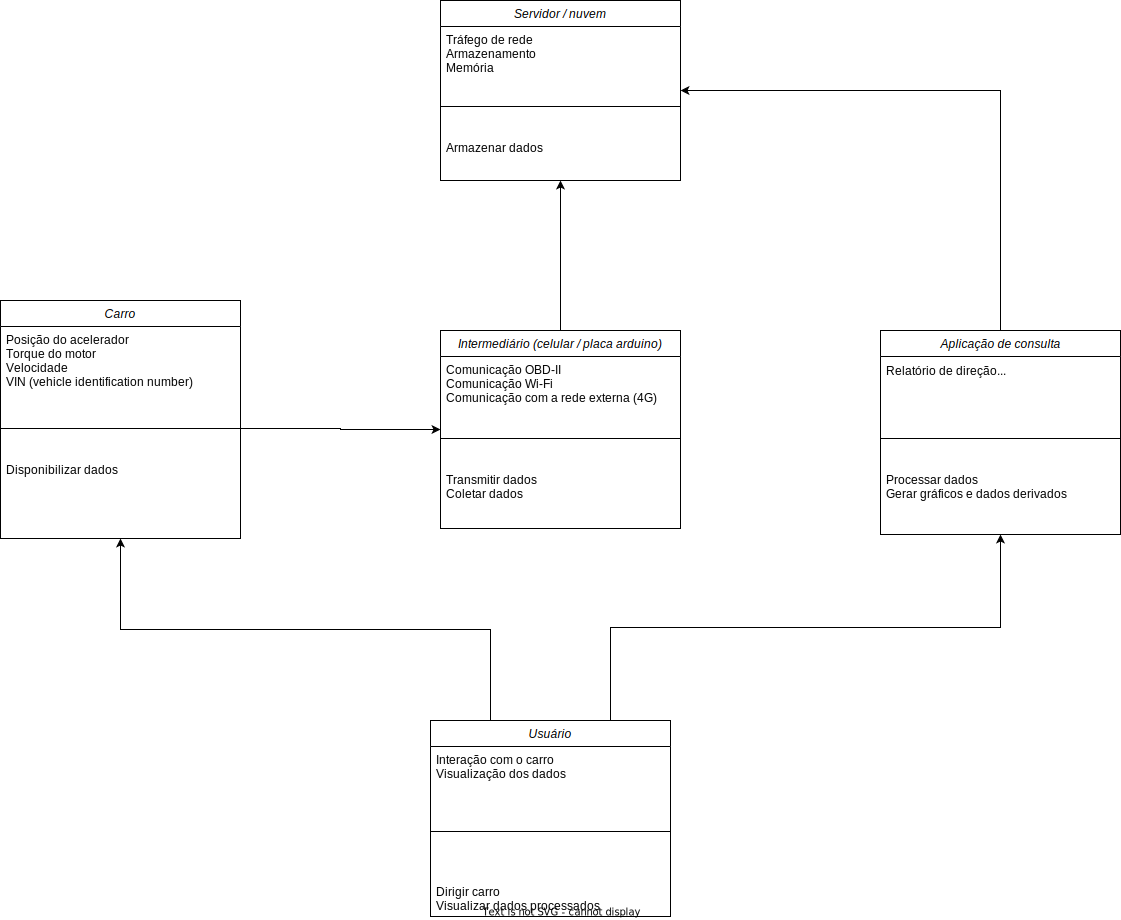
\includegraphics[scale=0.4]{figures/coleta_dados_carro}
    
    \caption{Diagrama de classes com visão mais abstrata do sistema}
    
    \label{fig:class_diagram}
\end{figure}

\section{Requisitos funcionais}
\begin{itemize}
    \item \textbf{Conexão OBD-II:} o aplicativo se comunica com a interface do carro, requisitando apenas as informações definidas, durante o projeto, como relevantes.
    
    \item \textbf{Conexão do celular à \textit{internet}:} transmissão de dados coletados para a nuvem.
    
    \item \textbf{Plataforma de recepção na nuvem:} armazenamento dos dados coletados todos na plataforma de \textit{cloud} definida.
    
    \item \textbf{Histórico de Rotas:} capacidade de armazenar e acessar informações detalhadas sobre os trajetos percorridos por um veículo ao longo do tempo; este recurso é crucial para oferecer aos usuários e administradores uma visão retrospectiva das atividades de um veículo, permitindo uma compreensão abrangente dos padrões de movimentação e comportamento de condução.
\end{itemize}

\section{Requisitos não-funcionais}

\begin{itemize}
    \item \textbf{Conexão contínua com a \textit{internet}:} conexão não para por muito tempo, análise contínua dos dados coletados.
    
    % , além de gerar desconfiança por parte do usuário, ao perceber que não há consistência no sistema.
    
    \item \textbf{Interface sem reconexão manual com a \textit{internet} e \textit{bluetooth}:} re-estabelecimento da conexão com o OBD e a \textit{internet} sem interferência do usuário assim que for ligada novamente; em outras palavras, um sistema \textit{plug and play}.
    
    \item \textbf{Informações relevantes e corretas:} dados apresentados no relatório de direção com nexo para o usuário; apenas meta-informações chegam ao usuário final, passando por "filtro de plausibilidade".
    
    % , para que, mais uma vez, a confiança de quem usará o sistema não seja perdida ao deparar-se com valores \textit{outliers} nas análises geradas.
    
    \item \textbf{Memória e armazenamento em nuvem suficientes:} espaço máximo em nuvem que pode ser usado claramente sinalizado para o usuário ao usar o sistema; além de sinalização de que suas informações não serão mais coletadas assim que o armazenamento seja ocupado por completo.
    
    \item \textbf{Segurança de dados:} pessoas não-autorizadas não podem ter acesso aos dados coletados no veículo de cada usuário.
\end{itemize}

% \subsection{}
% \subsection{}
% \subsection{}



\chapter{Desenvolvimento do trabalho}

% Apresentar os resultados das fases que transformam
% os requisitos em produtos finais.
% • A estrutura desse capítulo depende do processo de
% desenvolvimento do trabalho.
% • A organização e as seções desse capítulo devem ser
% definidas juntamente com o orientador.

Este capítulo tem como objetivo explicitar quais foram as decisões de projeto que foram tomadas ao longo do desenvolvimento do sistema.

\section{Justificativas das métricas escolhidas}

As escolhas das métricas para o desenvolvimento desse projeto foram determinantes para avaliar e interpretar resultados com precisão. As métricas escolhidas auxiliam a avaliar o perfil dos motoristas.

\subsection{RPM}

 Em um motor de combustão interna, o RPM indica a velocidade com que os pistões se movem para cima e para baixo no cilindro. O controle preciso do RPM é essencial para otimizar a eficiência do motor e a entrega de potência, sendo um indicador chave para os motoristas ajustarem suas velocidades de condução.

 A figura \ref{fig:rpmxpotencia} mostra que a potência aumentou com o aumento da rotação do motor\textsuperscript{[28]}. Operar consistentemente em RPMs muito altos pode levar a um aumento do desgaste mecânico, já que componentes como pistões, bielas e válvulas são submetidos a forças intensas em altas velocidades. Por outro lado, operar em RPMs muito baixos pode resultar em acúmulo de resíduos e combustão incompleta, afetando negativamente a eficiência do motor.

 \begin{figure}[hp]
    \centering
    
    \includegraphics[scale= 1]{figures/rpmxpotencia.jpeg}
    
    \caption{Potência versus velocidade do motor.}
    
    \label{fig:rpmxpotencia}
\end{figure}

\subsection{Trajetos e rotas perigosas}

A relação entre rotas perigosas, marcadas por assaltos e roubos de carros e o perfil do motorista tornam-se elementos críticos na gestão da segurança. A escolha da rota, desempenha um papel significativo na mitigação desses perigos. 

Motoristas que optam por passar frequentemente por áreas consideradas de alto risco podem estar mais suscetíveis a incidentes indesejados. Portanto, compreender o perfil do motorista em relação a essas rotas perigosas é importante para a implementação de estratégias eficazes de prevenção. A conscientização dos motoristas sobre áreas de risco podem contribuir para uma abordagem mais segura ao planejar e seguir rotas.
Locais como Paulista, Augusta e Sé possuem altos índices de furtos. A figura 

\begin{figure}[hp]
    \centering
    
    \includegraphics[scale=0.8]{figures/rotas_autorisco.jpeg}
    
    \caption{Gráfico da aceleração nos eixos x, y, z.}
    
    \label{fig:aceleracao}
\end{figure}

 
\section{Tecnologias utilizadas}
O projeto pretende definir algumas tecnologias de base para serem usadas durante o desenvolvimento de cada fase dele.

    \subsection{Amazon Web Services}

    A escolha da AWS para o projeto é fundamentada em três pilares essenciais: escalabilidade, segurança e viabilidade econômica. 
    
    A capacidade desse serviço de nuvem de se adaptar dinamicamente às demandas do sistema assegura uma infraestrutura flexível, capaz de lidar eficientemente com variações na carga de trabalho. 
    
    Além disso, a reputação consolidada da Amazon em termos de segurança oferece uma base robusta para proteção dos dados e operações. 
    
    Por fim, a viabilidade econômica se destaca, uma vez que a AWS disponibiliza uma variedade de serviços e modelos de precificação que se alinham de maneira eficaz às necessidades do projeto, otimizando custos operacionais.

    É evidente que todas essas vantagens só são concretizadas caso os implementadores do sistema façam uso de toda a funcionalidade da nuvem: projetos monolíticos, ainda que rodados em servidores distribuídos, não exploram a flexibilidade de serviços como a AWS. 

    \subsection{Conexão OBD-II}

    A integração do OBD-II (\textit{On-Board Diagnostics}) neste projeto de sistema de coleta de dados representa um avanço significativo na obtenção de dados precisos e abrangentes sobre o desempenho do veículo. O OBD-II, um padrão presente em muitos veículos modernos, fornece acesso a uma variedade de parâmetros, como velocidade, rotações por minuto (RPM), temperatura do motor, e códigos de diagnóstico de falhas. Ao conectar a plataforma de captura de dados ao conector OBD-II do veículo, é possível extrair informações em tempo real sobre a condução, condições do motor e possíveis problemas mecânicos.

    Já existe uma plataforma aceleradora desenvolvida no GitHub que consegue comunicar-se com o veículo através do protocolo OBD-II\textsuperscript{[12]}. 
    
    Esse outro projeto implementa o protocolo OBD-II e também uma interface gráfica básica para mostrar os dados fornecidos pelo carro.

    A figura \ref{fig:obd2_plataforma} mostra uma plataforma onde é possível ver alguns dos dados quando o motorista estava dando uma volta ao redor do bairro.

\begin{figure}[hp]
    \centering
    
    \includegraphics[scale=0.3]{figures/obd2.jpg}
    
    \caption{Interface básica com porta OBD-II\textsuperscript{[12]}.}
    
    \label{fig:obd2_plataforma}
\end{figure}
    
    \subsection{Android Studio} A utilização da IDE Android Studio neste projeto de sistema de coleta de dados desempenha um papel central no desenvolvimento de aplicativos móveis dedicados à interação com o sistema. 
    
    O Android Studio, sendo a principal ferramenta de desenvolvimento para aplicativos Android, oferece um ambiente integrado e robusto que simplifica a criação, teste e depuração de software. 
    
    A plataforma fornece recursos avançados de design de interface do usuário, facilitando a criação de aplicativos intuitivos e visualmente atraentes para os usuários finais. A integração perfeita com o Android SDK (Software Development Kit) permite o acesso às APIs e recursos específicos do sistema operacional Android, garantindo uma implementação eficiente de funcionalidades como a transmissão Bluetooth, a visualização de dados de rastreamento e a interação em tempo real. 
    
    Além disso, as ferramentas de emulação e depuração incorporadas no Android Studio simplificam o processo de teste em diferentes dispositivos, contribuindo para a criação de aplicativos estáveis e adaptáveis.

    Por último, nenhuma tecnologia multiplataforma (React Native ou Flutter, por exemplo) ou específica de dispositivos iOS (Swift ou Objective C, por exemplo) foi escolhida, pois o intuito do projeto era ser compatível com os celulares dos membros do grupo e devido à familiaridade com a linguagem Java, usada para esse tipo de desenvolvimento.

     \begin{figure}[hp]
    \centering
    
    \includegraphics[scale=0.4]{figures/logo_android.png}
    
    \caption{Logo Android Studio.}
    
\end{figure}
    
     \subsection{Banco de dados} A integração do MySQL e do AWS RDS (Relational Database Service) em um projeto de sistema de compilação de dados de veículos é uma estratégia robusta para o gerenciamento eficiente e escalável dos dados do sistema. O MySQL, um sistema de gerenciamento de banco de dados relacional de código aberto, proporciona uma estrutura confiável para armazenar e organizar informações como histórico de rotas e dados do OBD-II. 
     
     Ao escolher o AWS RDS como a plataforma de hospedagem para o MySQL, ganha-se os benefícios adicionais de escalabilidade automática, alta disponibilidade e segurança avançada oferecidos pela infraestrutura em nuvem da Amazon. A integração dessas tecnologias permite o acesso eficiente aos dados, consultas rápidas e uma gestão simplificada do banco de dados. 
     
     Além disso, o AWS RDS lida com tarefas operacionais, como backup automático e manutenção, permitindo que os desenvolvedores concentrem seus esforços em aprimorar as funcionalidades do sistema de rastreamento. 
     
     Essa combinação proporciona uma base sólida para o armazenamento e recuperação de dados, promovendo a confiabilidade e eficácia do sistema.

     A estrutura definida para as tabelas do banco de dados foi:


    \begin{itemize}
         \item{\textbf{tcc-schema} (esquema do banco de dados onde se encontram as tabelas)}
         
        \begin{itemize}
             \item{\textbf{info:} Armazena as informações coletadas através da porta OBD} 
        
             \item{\textbf{acceleration:} Contém dados dos acelerômetros do celular do usuário} 
             
             \item{\textbf{location:} Guarda latitude e longitude obtidas por GPS pelo celular}   
        \end{itemize}  
    \end{itemize}

     A especificação exata das colunas de cada tabela pode ser encontrada no apêndice. [MENCIONAR APENDICE POR NUMERO]

    \begin{figure}[hp]
        \centering
        
        \includegraphics[scale=0.4]{figures/logo_Mysql.jpg}
        
        \caption{Logo do Mysql.}
        
    \end{figure}

    
     \subsection{\textit{Python} e Folium} A junção do Python e do Folium em um projeto de sistema de coleta de dados oferece uma poderosa combinação para a visualização interativa e geoespacial dos dados. O Folium é uma biblioteca Python que simplifica a criação de mapas interativos baseados na web, utilizando a infraestrutura do Leaflet.js. Integrar o Folium ao projeto permite que os desenvolvedores gerem mapas dinâmicos que destacam informações específicas relacionadas ao rastreamento de veículos.

    Essa integração Python-Folium é particularmente útil para análises geoespaciais em sistemas de rastreamento de veículos, proporcionando uma representação geográfica e visualmente intuitiva dos dados de telemetria. 
    
    A flexibilidade do Python permite a personalização dos mapas e a incorporação de recursos adicionais conforme as necessidades específicas do projeto, contribuindo para uma interface de usuário mais informativa e envolvente.

      \begin{figure}[hp]
    \centering
    
    \includegraphics[scale=0.1]{figures/python_folium.jpg}
    
    \caption{Logo Python + Folium.}
\end{figure}

% interface com usuario, banco de dados, conexão obd2

    \subsection{Flask}

    A seleção da biblioteca Flask para o projeto ocorreu devido à familiaridade com a linguagem Python, tornando o desenvolvimento mais acessível. Adicionalmente, a escolha se fundamentou na capacidade do Flask em facilitar a implementação eficiente de uma API, atendendo à necessidade do aplicativo de enviar e receber dados de maneira eficaz. O código python da API em Flask foi hospedado em um Lambda da AWS para facilitar o seu uso pelo APP posteriormente.


\section{Projeto e implementação}
% Esta seção descreverá as decisões feitas durante o trabalho.

\subsection{Folium}
    Para criar os mapas do aplicativo, foi utilizado o \textit{framework} Folium. Essa biblioteca é uma poderosa ferramenta para manipular e visualizar dados geoespaciais usando Python. 
    
    Com o Folium, é possível criar mapas interativos personalizados e incorporar dados neles de várias maneiras. Para manipular dados usando essa ferramenta, pode-se começar importando a biblioteca e criando um objeto Map que representa o mapa. 
    
    Em seguida, pode-se adicionar camadas, como marcadores, polígonos e \textit{popups}, para exibir dados de forma intuitiva no mapa. 
    
    % O Folium permite a integração de dados geoespaciais em diferentes formatos, como GeoJSON, tornando-o uma ferramenta flexível para análise e visualização de dados geoespaciais em Python. 
    
    A figura 
    \ref{fig:python_libs} mostra as bibliotecas utilizadas para desenvolver os mapas do projeto.
    
    \begin{figure}[hp]
        \centering
        
        \includegraphics[scale=0.8]{figures/bibliotecas.jpg}
        
        \caption{Bibliotecas utilizadas para gerar o mapa da rota do usuário.}
        
        \label{fig:python_libs}
    \end{figure}
    
            % \begin{center}
            %  \includegraphics[scale=0.8]{figures/bibliotecas.jpg}
            %  
            %  \end{center}
            
    Para traçar uma trajetória no mapa usando a biblioteca Folium em Python, será necessário uma lista de pontos de latitude e longitude que representam a trajetória. A partir dos pontos de latitude e longitude colhidos dos sensores do celular, cria-se uma lista de coordenadas que representam os pontos da trajetória. Em seguida, criamos um objeto de mapa usando o Folium e é adicionado uma linha de trajetória (um polilinha) que conecta os pontos da lista e o mapa pode ser visualizado. Uma demonstração de uma trajetória pode ser vista na figura \ref{fig:car_route_1}.
    
    \begin{figure}[hp]
        \centering
        
        \includegraphics[scale=0.8]{figures/rota_1.jpg}
        
        \caption{Rota de uma das viagens fornecidas pelo \textit{UAH Driveset}.}
        
        \label{fig:car_route_1}
    \end{figure}
    
    A visualização de um vídeo que apresenta o trajeto do veículo sincronizado com um gráfico de aceleração proporciona uma compreensão visual e analítica aprimorada do comportamento de condução. Este recurso permite aos usuários acompanhar de forma imersiva o percurso do veículo enquanto simultaneamente observam as variações na aceleração ao longo do tempo. 
    
    Ao visualizar o vídeo, os usuários podem identificar eventos específicos, como curvas acentuadas, frenagens bruscas ou acelerações rápidas, correlacionando-os diretamente com os picos e quedas no gráfico de aceleração exibido ao lado. Essa abordagem oferece uma representação mais holística da experiência de condução, permitindo uma análise detalhada de como o estilo de direção afeta diretamente a aceleração do veículo. 
    
    Além disso, essa visualização combinada pode ser uma ferramenta valiosa para treinamento de motoristas, análise de incidentes e \textit{feedbacks} personalizados, proporcionando uma compreensão mais rica e envolvente do desempenho do veículo e do comportamento do condutor.

    \subsection{Análise de Dados - RideParser}\label{rideparser}

    A função da classe RideParser é analisar dados dos trajetos feitos pelos motoristas. 
    
    Alguns filtros são recebidos pelo construtor dessa classe, para personalizar a geração de gráficos. Esses parâmetros são usados para restringir o que vem do banco de dados a uma certa janela de tempo e ao usuário que solicita aquela informação.
    
    % Já o módulo 
    % ''os'' fornece funcionalidades relacionadas ao sistema operacional, permitindo que você interaja com o ambiente do sistema, como manipular diretórios, arquivos, obter informações sobre o sistema, manipular variáveis de ambiente, entre outras tarefas relacionadas ao sistema operacional.
    Dentro desse mesmo arquivo, algumas bibliotecas típicas de ciência de dados foram utilizadas para manipular os gráficos mencionados. Foram elas: pandas, matplotlib, numpy e scipy.
    
    A figura \ref{fig:rota1integrante} mostra o video e o gráfico da aceleração.
    
    \begin{figure}[hp]
        \centering
        
        \includegraphics[scale=0.3]{figures/rota_integrante.jpg}
        
        \caption{Rota de uma viagem de um dos integrantes do grupo.}
        \label{fig:rota1integrante}
    \end{figure}

    \subsection{API Rest - Flask}
    A implementação da API centraliza-se em uma arquitetura Python utilizando a biblioteca Flask, proporcionando uma estrutura ágil e eficiente para a comunicação com a base de dados MySQL, hospedada em um serviço de RDS na AWS. A escolha da linguagem Python e do framework Flask foi motivada pela sua simplicidade e flexibilidade, permitindo a rápida construção dos endpoints responsáveis pela interação entre o aplicativo e a base de dados.

    A lógica da API foi encapsulada em funções específicas, acionadas por meio de requisições POST. O corpo do JSON enviado nessas requisições determina a ação a ser executada, que pode ser uma entre seis operações distintas. Três destas operações referem-se a consultas (GET) e três a modificações (POST), cada uma vinculada a uma das três tabelas da base de dados.

    Para facilitar a utilização da API pelo app, o código Python foi integrado ao ambiente serverless da AWS Lambda. Essa escolha estratégica permite que as funções sejam invocadas sob demanda, proporcionando uma resposta ágil às requisições do aplicativo Android, que, por sua vez, está sendo desenvolvido no ambiente Java do Android Studio. A combinação dessas tecnologias promove uma arquitetura eficiente para gerenciar a comunicação entre o aplicativo e a infraestrutura de banco de dados na nuvem.


    \subsection{Criação de relatório em PDF}
    
    A geração de insights visuais e análise métrica a partir dos dados armazenados na base MySQL é um componente essencial do projeto. A decisão de fazer isso através da geração de um PDF para o motorista baseou-se na clareza e simplicidade desse formato de arquivo. Essa escolha é respaldada também pela facilidade de implementação, disponibilizada pela biblioteca \textit{Matplotlib}, que permite a criação de PDFs formatados contendo os gráficos com as métricas geradas.
    
    Um segundo AWS Lambda desempenha um papel central nesse processo, funcionando como uma ponte entre a base de dados e as ferramentas de visualização. Ao ser acionado, esse Lambda realiza uma chamada ao outro Lambda, que extrai as informações relevantes da base de dados MySQL referentes ao usuário, para realizar a análise.

    Utilizando a biblioteca Matplotlib em Python, a função Lambda então emprega métodos da classe RideParser, mencionada na sessão \ref{rideparser}, para criar um relatório do motorista, com gráficos e métricas relevantes referentes a sua condução. Isso proporciona aos usuários uma compreensão mais aprofundada das métricas associadas às suas atividades.
    
    Para proporcionar aos usuários uma maneira acessível de interagir com esses insights, um botão "gerar PDF" foi incorporado no aplicativo. Este botão aciona o segundo Lambda, que compila os gráficos e métricas gerados em um arquivo PDF. A utilização da biblioteca smtplib facilita o envio desse PDF diretamente para o usuário via email. Essa solução integrada oferece uma experiência completa aos usuários, permitindo-lhes não apenas visualizar, mas também compartilhar os resultados de suas análises de maneira eficaz.    

    \subsection{Autenticação com \textit{Firebase}}

    A  escolha do \textit{Firebase} para a identificação única do usuário no sistema decorre da capacidade da plataforma em oferecer eficiência e segurança nesse processo, diminuindo-se a carga de responsabilidade do sistema em armazenar informações sensíveis de cada pessoa. 
    
    Essa decisão é fundamentada pela praticidade proporcionada pela integração do \textit{Firebase} com aplicativos \textit{Android} e páginas web\textsuperscript{[29]}, simplificando a implementação de autenticação e gestão de usuários, assegurando uma identificação singular e segura no âmbito do sistema em questão.

    \subsection{Dependências do Gradlle}

    Em um primeiro instante o app android-obd-reader não queria rodar na IDE Android studio. Para que isso fosse possível foi necessario fazer alterações no arquivo \textbf{gradle/wrapper/gradle-wrapper.properties}. Atualizar as dependências do Gradle  é muitas vezes necessário para garantir que o seu aplicativo possa se beneficiar das correções de bugs, melhorias de desempenho e novos recursos fornecidos pelas versões mais recentes das bibliotecas que você está utilizando. Este link \url{https://github.com/APF2000/android-obd-reader-pires/commit/def70ed262b1fad28cc9e2b98a48af45cfac5695} mostra as alterações que foram necessárias.

    \subsection{Proteção dos dados}
    
    Na Lei Geral de Proteção de Dados (Lei n. 13.709/18-LGPD), parte-se da ideia de que todo dado pessoal tem importância e valor. Por essa razão se adotou conceito amplo de dado pessoal, assim como estabelecido no Regulamento europeu \textsuperscript{[30]} (GDPR-General Data Protection  Regulation). Quando se trata de um aplicativo projetado para analisar o perfil do motorista de carros, a LGPD impõe uma série de responsabilidades e requisitos ao desenvolvedor e operador do aplicativo. É necessário obter o consentimento  do usuário antes de coletar e processar quaisquer dados pessoais relacionados ao seu perfil de condução.
    
    Além disso, a LGPD exige que medidas de segurança apropriadas sejam implementadas para proteger esses dados contra acessos não autorizados e vazamentos. Os usuários têm o direito de acessar, corrigir e excluir suas informações pessoais, e o aplicativo deve fornecer meios para que esses direitos sejam exercidos.


% Using \texttt{biblatex} you can display a bibliography divided into sections, depending on citation type. 
% Let's cite! Einstein's journal paper \cite{einstein} and Dirac's book \cite{dirac} are physics-related items. 
% Next, \textit{The \LaTeX\ Companion} book \cite{latexcompanion}, Donald Knuth's website \cite{knuthwebsite}, \textit{The Comprehensive Tex Archive Network} (CTAN) \cite{ctan} are \LaTeX-related items; but the others, Donald Knuth's items, \cite{knuth-fa,knuth-acp} are dedicated to programming. 




\section{Testes e avaliação}
% descrever o plano de testes do sistema: testes de software, modulo, integração e validação
Alguns testes foram definidos para a ratificação das funcionalidades do sistema:

\begin{itemize}
    \item \textbf{Conferir conexão OBD-II:} 
    
    \begin{itemize}
        \item Conectar o dispositivo de leitura na entrada do carro
        \item Ligar a comunicação \textit{bluetooth} do celular
        \item Parear os dois dispositivos
        \item Digitar a senha 1234, padrão dos dispositivos de leitura OBD
        \item Ligar a coleta de dados através do aplicativo
        \item A tela deve sinalizar que o protocolo está sendo feito da forma correta
    \end{itemize}
    
    \item \textbf{Teste de continuidade de transferência de dados:} 
    \begin{itemize}
        \item Fazer conexão com o OBD conforme descrito no teste anterior
        \item Andar com o carro por alguns minutos com a tela do celular desbloqueada (de preferência mudar o \textit{timeout} da tela nas configuraçõs do celular)
        \item Atestar que nenhum dado foi perdido por falta de conexão (pode ser visto por descontinuidade dos gráficos)
    \end{itemize}
    
    \item \textbf{Equivalência de envio e recepção de dados:}
    \begin{itemize}
        \item Comparar o \textit{log} de envio de dados do aplicativo de interface com a porta OBD-II com o \textit{log} de salvamento do banco de dados hospedado na nuvem
        \item A quantidade de dados, os \textit{timestamps} deles e seus conteúdos devem ser idênticos
    \end{itemize}
    
    \item \textbf{Testes de segurança:} 
    \begin{itemize}
        \item Ratificar que não é possível ter acesso aos dados de um certo usuário sem ter as informações de \textit{login}
        \item Verificar o certificado SSL do remetente e só aceitar a mensagem se a informação condisser com as credenciais armazenadas daquele usuário
    \end{itemize}
    
    \item \textbf{Geração de dados \textit{outliers}:}
    \begin{itemize}
        \item Verificar se o sistema descarta corretamente as informações que fogem totalmente do padrão esperado ou se consegue pelo menos esconder isso do usuário
        \item Os PDFs gerados com o sistema devem sofrer um processo de análise de plausibilidade, o que deve averiguar que a análise automática está sendo feita corretamente
    \end{itemize}
    
\end{itemize}


\subsection{Fluxo de uso do sistema}

    \begin{itemize}
    \item \textbf{Autenticação com o Google:}
    O aplicativo no celular deve ser iniciado para realizar a autenticação com as credenciais do Google, assegurando uma identificação segura do usuário.

    \item \textbf{Conexão com o OBD:}
    A conexão entre o celular e o OBD deve ser estabelecida, garantindo que o leitor esteja corretamente emparelhado para iniciar a comunicação.

    \item \textbf{Início da Coleta de Dados:}
    A coleta de dados deve ser ativada por meio do aplicativo.

    \item \textbf{Condução do Veículo:}
    O veículo deve ser conduzido normalmente, permitindo que o aplicativo faça a coleta de dados em tempo real.

    \item \textbf{Posicionamento Fixo do Celular:}
    O celular deve ser fixado em uma posição estável dentro do veículo usando um suporte apropriado. Isso garantirá que os dados de aceleração sejam confiáveis, o que evitará qualquer tipo de interferência na análise posterior da direção.
\end{itemize}


\subsection{Carros utilizados para teste}

    A escolha dos carros onde o leitor de OBD seria conectado foi feita a partir dos veículos de familiares.

    Os modelos em que o sistema foi testado, foram em maioria para analisar quais parâmetros de OBD haviam sido implementados em todos eles.

    Os carros usados foram:

    \begin{itemize}
        \item Hyundai Ix35 - 2012
        \item Mercedes C200 CGI - 2014
        \item Ford Xsport - 2008
    \end{itemize}

    O modelo Ix35 foi a principal fonte de dados do projeto, pois praticamente todos os testes feitos para a nova base de dados foram feitos com ele.

    \subsection{Aparelhos \textit{smartphone}}

    O aplicativo foi rodado em dois modelos diferentes de celular:
    \begin{itemize}
        \item Samsung Galaxy A71
        \item Samsung Note S22
    \end{itemize}


\chapter{Considerações finais}

Este capítulo descreve as observações posteriores à conclusão do projeto.

\section{Conclusões do projeto de formatura}
% "foi bom, tivemos que mudar isso e isso e isso"
Esta seção será modificada quando o projeto tiver sido implementado.

\section{Contribuições}
% qual foi a contrib da equipe
Esta seção será modificada quando o projeto tiver sido implementado.

\section{Perspectivas de continuidade}
% o que pode ser feito depois do tcc?
Embora o projeto ainda não tenha acabado, já é possível vislumbrar o que pode ser feito com o sistema que será desenvolvido.

A ideia principal dos itens listados a seguir é a de fazer uso da plataforma de dados como ferramenta principal de fornecimento de dados:

\begin{itemize}
    \item \textbf{Classificador de perfil de direção para seguros de carro personalizados:} valores mais altos para motoristas mais violentos.
    
    \item \textbf{Prova de direção conduzida por Inteligência Artificial:} possível supressão da prova do Detran, avaliando o condutor ao longo das aulas práticas.
    
    \item \textbf{Ranqueador de segurança de carros autônomos:} avaliação dos carros do futuro para determinar qual dirige com mais segurança.
    
    \item \textbf{Revisão remota / diagnóstico automático de carro:} relatar problemas antes que aconteçam, sem a necessidade de um mecânico para examinar diretamente o veículo.
    
    \item \textbf{Classificação de motoristas de aplicativo:} avaliação ponderada pela forma de dirigir
\end{itemize}
\chapter{Apêndices}

% Como juntar todas as subpartes do projeto é uma outra tarefaimportante de engenharia.

% A seguir é descrito como isso pode ser feito.

%%%%%%%%%%%%%%%%%%%

\section{Conversa com um profissional da Porto Seguro sobre seguros de carro}

%%%%%%%%%%%%%%%%%%%

\noindent
\textbf{Pergunta 1:} 
Quanto aos locais por onde o motorista passa ao longo do dia, é mais importante saber o nome do bairro por onde ele passa ou se soubermos a rua é melhor pra sabermos o risco de assalto?

\noindent
\textbf{Resposta 1:} 
A precificação do seguro já é baseada em três fatores: onde a pessoa mora, onde ela trabalha e o trajeto feito por ela para ir de um local ao outro.
Na nossa plataforma, chamada \textit{Corretor Online}, temos acesso a esses e outro dados do cliente, o que nos possibilita precificar o seguro de forma personalizada.

%%%%%%%%%%%%%%%%%%%

\noindent
\textbf{Pergunta 2:} 
É importante a hora em que a pessoa passa em cada lugar? Ou dia da semana é um fator mais determinístico?

\noindent
\textbf{Resposta 2:}
Não há correlação provada entre o dia da semana em que a pessoa dirige e a probabilidade de acidente de carro.

A hora do dia, no entanto, como pode ser intuitivo para muitos, determina a chance de o carro ser roubado. A maior parte dos crimes ocorre à noite.

%%%%%%%%%%%%%%%%%%%

% \textbf{Pergunta 3:} Momentos com mais trânsito podem ser um fator de risco para acidentes?


%%%%%%%%%%%%%%%%%%%

\noindent
\textbf{Pergunta 3:} O sistema de precificação por uso é interessante pra seguros de motoristas de aplicativos? Quais parâmetros são mais relevantes para quem usa o carro prolongadamente?

\noindent
\textbf{Resposta 3:}
Sim, com certeza seria interessante um sistema desse tipo.

\noindent
Sobre os parâmetros exatos que seriam mais interessantes, preciso consultar a área estatística da empresa para ter mais certeza, mas certamente informações sobre como o motorista usa o carro (a quantidade de freadas bruscas ao longo do trajeto, por exemplo) e por onde passa com ele, conforme mencionei anteriormente, são fundamentais, na minha experiência.

%%%%%%%%%%%%%%%%%%%

\noindent
\textbf{Pergunta 4:} 
Empresas podem se beneficiar da redução do seguro também? Levando-se em conta viagens feitas por funcionários, a trabalho

\noindent
\textbf{Resposta 4:}
Hoje em dia nós seguramos empresas baseado puramente em quanto veículos têm na frota delas e quanto eles serão usados em média.

\noindent
Se fosse possível diferenciar um motorista do outro, o cálculo do risco seria mais preciso, além de poder incentivar a boa condução.

\noindent
Fizemos uma campanha com ideia parecida uma vez, chamada \textit{Trânsito Mais Gentil}. A ideia era diminuir o prêmio cobrado de cada segurado caso ele comprovasse, ao fim do ano, que cometeu poucas ou nenhuma infração no trânsito, dando-nos a quantidade de pontos recebidos na carteira.

%%%%%%%%%%%%%%%%%%%
    
\noindent
\textbf{Pergunta 5:} 
Existe o interesse de ser feita uma precificação mais personalizada de seguros de carro, usando-se dados de estilo de direção de cada indivíduo em vez de estatísticas gerais?

\noindent
\textbf{Resposta 5:}
Definitivamente sim, e acredito que essa seja a tendência do mercado no futuro próximo.

\noindent
Existe uma plataforma que implementa algo parecido com o que vocês estão desenvolvendo, chama-se Azos\textsuperscript{[30]}.

\noindent
Essa empresa precifica seguros de vida de forma dinâmica, levando em consideração não apenas estatísticas gerais sobre doenças que cada pessoa pode desenvolver, mas também e principalmente os hábitos do dia a dia de cada um e quais as novas condições de saúde do segurado a cada renovação de contrato.

%%%%%%%%%%%%%%%%%%%
    
\noindent
\textbf{Pergunta 6:} 
Alguma consideração final?
    
\noindent
\textbf{Resposta 6:} 
Quanto mais ajustado ao verdadeiro risco, melhor será o produto tanto para o cliente como para a seguradora, pois o preço mais justo para aquele serviço será o efetivamente cobrado.

\noindent
Dito isso, vejo com muito bons olhos o projeto de vocês e contribuo com uma sugestão: algo tão personalizado assim poderia implementar um sistema equivalente ao \textit{Open Banking}, de que tanto se fala hoje em dia, uma vez que o histórico de cada cliente não é transferível entre empresas de seguro.

%%%%%%%%%%%%%%%%%%%


\section{Colunas da tabela do banco de dados}

\begin{python}
CREATE TABLE `tcc_main`.`info` (
  `id` INT NOT NULL AUTO_INCREMENT, 
  `timestamp` TIMESTAMP(3) NOT NULL,
  `user_token` VARCHAR(40),
  `name` VARCHAR(45) NOT NULL,
  `result` VARCHAR(45) NOT NULL,
  PRIMARY KEY (`id`),
  UNIQUE INDEX `id_UNIQUE` (`id` ASC) VISIBLE);

CREATE TABLE `acceleration` (
  `id` INT NOT NULL AUTO_INCREMENT,
  `timestamp` TIMESTAMP(3) NOT NULL,
  `user_token` VARCHAR(40),
  `acceleration_x` VARCHAR(10) NOT NULL,
  `acceleration_y` VARCHAR(10) NOT NULL,
  `acceleration_z` VARCHAR(10) NOT NULL,
  `gravity_x` VARCHAR(10) NOT NULL,
  `gravity_y` VARCHAR(10) NOT NULL,
  `gravity_z` VARCHAR(10) NOT NULL,
  PRIMARY KEY (`id`),
  UNIQUE INDEX `id_UNIQUE` (`id` ASC) VISIBLE);

CREATE TABLE `location` (
  `id` INT NOT NULL AUTO_INCREMENT,
  `timestamp` TIMESTAMP(3) NOT NULL,
  `user_token` VARCHAR(40),
  `latitude` VARCHAR(20) NOT NULL,
  `longitude` VARCHAR(20) NOT NULL,
  PRIMARY KEY (`id`),
  UNIQUE INDEX `id_UNIQUE` (`id` ASC) VISIBLE);

\end{python}


%%%%%%%%%%%%%%%%%%%%%%%%%%%%%%%



\section{Código para o Lambda da AWS de comunicação com o banco de dados}

\begin{python}

import awsgi
import pymysql
from flask import Flask, request

app = Flask(__name__)

@app.route("/app_data", methods=["POST"])
def api_data():
    host = "open-db.clznpmxaqrkl.us-east-1.rds.amazonaws.com"
    user = "testadm"
    password = "testadm#1"
    database = "tcc_schema"
    
    #Connection
    connection = pymysql.connect(host=host, user=user, 
    password=password, database=database)
    cursor = connection.cursor()

    data = request.get_json()
    
    method_name = data["method"]

    if method_name.split("_")[0] == "get" :
        filters = {
            "time_min" : data["time_min"],
            "time_max" : data["time_max"],
            "user_token" : data["user_token"]
        }
        
    data = data.get("data", [])

    if(method_name == "add_obd_info"):
        print("inserto data to info")

        query_insert_cmd = "INSERT INTO info (timestamp, user_token, name, 
        result) VALUES (\%(timestamp)s, \%(user_token)s, \%(name)s, \%(result)s)"
        cursor.executemany(query_insert_cmd, data)

        connection.commit()
        return "deu bom"
    
    elif(method_name == "add_acceleration"):
        print("insert data to acceleration")

        query_insert_cmd = "INSERT INTO acceleration (timestamp, user_token, 
        acceleration_x, acceleration_y, acceleration_z, gravity_x, gravity_y, 
        gravity_z) VALUES (\%(timestamp)s, \%(user_token)s, \%(acceleration_x)s,
        \%(acceleration_y)s, \%(acceleration_z)s, \%(gravity_x)s, \%(gravity_y)s,
        \%(gravity_z)s)"
        cursor.executemany(query_insert_cmd, data)

        connection.commit()
        return "deu bom"
    
    elif(method_name == "add_location"):
        print("insert data to location")

        query_insert_cmd = "INSERT INTO location (timestamp, user_token,
            latitude, longitude) VALUES (\%(timestamp)s, \%(user_token)s, 
            \%(latitude)s, \%(longitude)s)"
        cursor.executemany(query_insert_cmd, data)

        connection.commit()
        return "deu bom"
    
    elif(method_name == "get_obd_info"):
        print("get data from info")
        
        query_select_cmd = "SELECT * FROM info where timestamp >= 
            '\%(time_min)s' and timestamp <= '\%(time_max)s' 
            and user_token = '\%(user_token)s'" \%filters

        cursor.execute(query_select_cmd)

        return {"data": cursor.fetchall()}
    
    elif(method_name == "get_acceleration"):
        print("get data from acceleration")

        query_select_cmd = "SELECT * FROM acceleration where timestamp >= 
            '\%(time_min)s' and timestamp <= '\%(time_max)s' 
            and user_token = '\%(user_token)s'" \% filters
        cursor.execute(query_select_cmd)

        return {"data": cursor.fetchall()}
    
    elif(method_name == "get_location"):
        print("get data from location")

        query_select_cmd = "SELECT * FROM location where timestamp >= 
            '\%(time_min)s' and timestamp <= '\%(time_max)s' 
            and user_token = '\%(user_token)s'" \%filters
        cursor.execute(query_select_cmd)

        return {"data": cursor.fetchall()}
    else:
        return {"status": "error, route not found"}

if __name__ == "__main__":
    app.run(debug=True, port=5000)


def lambda_handler(event, context):
    return awsgi.response(app, event, context)

\end{python}



%%%%%%%%%%%%%%%%%%%%%%%%%%%%%%%



\section{Código para o Lambda da AWS de geração do relatório sobre o perfil do motorista}

\begin{python}

import awsgi
from flask import Flask, request

import requests
import json

import matplotlib.pyplot as plt
from svglib.svglib import svg2rlg

import smtplib
from email.mime.multipart import MIMEMultipart
from email.mime.text import MIMEText
from email.mime.application import MIMEApplication

from io import BytesIO
from reportlab.lib.pagesizes import letter
from reportlab.lib import utils
from reportlab.platypus import SimpleDocTemplate, Paragraph, Image
from reportlab.lib.styles import getSampleStyleSheet

from ride_parser import RealRideParser


app = Flask(__name__)

@app.route("/create_pdf", methods=["POST"])
def app_pdf():
    data = request.get_json()

    body_json_obd_info = {
        "method": "get_obd_info",
        "time_min" : data["time_min"],
        "time_max" : data["time_max"],
        "user_token" : data["user_token"]
    }

    body_json_acceleration = {
        "method": "get_acceleration",
        "time_min" : data["time_min"],
        "time_max" : data["time_max"],
        "user_token" : data["user_token"]
    }

    body_json_location = {
        "method": "get_location",
        "time_min" : data["time_min"],
        "time_max" : data["time_max"],
        "user_token" : data["user_token"]
    }

    data_obd_info = get_data_from_lambda(body_json_obd_info)
    data_acceleration = get_data_from_lambda(body_json_acceleration)
    data_location = get_data_from_lambda(body_json_location)


    params = {
        "user_id" : data["user_token"],
        "date_beg" : data["time_min"],
        "date_end" : data["time_max"]
    }

    ride_parser = RealRideParser(True, **params)
    metrics_map = ride_parser.generate_pdf_metrics()
    img = ride_parser.risk_table_graph

    fig = plt.figure(figsize=(4, 3))
    plt.plot([1,2,3,4])
    plt.ylabel('some numbers')

    create_PDF(img)
    return("pdf criado")



def get_data_from_lambda(body_json):
    url = "https://pntdpvkdsc.execute-api.us-east-1.amazonaws.com/default/app_data"

    headers = {
        'Content-Type': 'application/json',
    }

    response = requests.post(url, headers=headers, data=json.dumps(body_json))

    if response.status_code == 200:
        print("data successfully obtained from the server")
        return response
    else:
        print("failed to get data from the server")
        

def send_email(recipient_email, pdf_buffer):
    # Configurações do e-mail
    sender_email = "gabiru.bx@gmail.com"
    sender_password = "vbwiquhkjpjsmwdu"
    subject = "test email pdf"

    # Configuração do server SMTP do Gmail
    server_smtp = "smtp.gmail.com"
    port_smtp = 587

    # Criação do objeto MIMEMultipart
    message = MIMEMultipart()
    message["From"] = sender_email
    message["To"] = recipient_email
    message["Subject"] = subject

    # Adiciona o corpo do e-mail (opcional)
    corpo_email = "Corpo do teste pdf"
    message.attach(MIMEText(corpo_email, "plain"))

    # Adiciona o arquivo PDF como anexo
    attached_document = MIMEApplication(pdf_buffer.read(), _subtype="pdf")
    attached_document.add_header(
        "Content-Disposition", f"attachment; filename=anexo.pdf")
    message.attach(attached_document)

    # Inicia a conexão com o server SMTP
    print("starting server")
    server = smtplib.SMTP(server_smtp, port_smtp)
    server.starttls()

    # Efetua login no server
    server.login(sender_email, sender_password)

    print("sending email")
    # Envia o e-mail
    server.sendmail(sender_email, recipient_email, message.as_string())

    # Fecha a conexão com o server
    server.quit()

def create_PDF(metrics_map):
    # Create a PDF document
    pdf_buffer = BytesIO()
    doc = SimpleDocTemplate(pdf_buffer, pagesize=letter)

    # Define a style sheet
    styles = getSampleStyleSheet()

    # Create a list of paragraphs for the content
    content = []

    # Add title
    content.append(Paragraph("My Data Report", styles['Title']))

    # Add space
    content.append(Paragraph("<br/>", styles['BodyText']))

    # Salvar a figura em um buffer de bytes
    metrics_map.savefig(pdf_buffer, format='png')
    pdf_buffer.seek(0)

    drawing=svg2rlg(pdf_buffer)

    doc.build(content)

    # Reset the buffer position to the beginning before sending
    pdf_buffer.seek(0)

    send_email("gabriel.morghett@gmail.com", pdf_buffer)

if __name__ == "__main__":
    app.run(debug=True, port=5000)

def lambda_handler(event, context):
    return awsgi.response(app, event, context)

\end{python}

\section{Conversão de coordenadas geográficas em índices dos blocos no mapa}

\begin{python}
def convert_coord_to_chunk(self, coord_1, coord_2, max_coord_diff):
    coord_diff = coord_1 - coord_2
    chunk = (self.segmentation_rate * coord_diff) // max_coord_diff
    return chunk

    self.north = car_crimes_df["latitude"].max() + (0.5 / 111.11)
    self.south = car_crimes_df["latitude"].min() - (0.5 / 111.11)
    self.west = car_crimes_df["longitude"].max() + (0.5 / 111.11)
    self.east = car_crimes_df["longitude"].min() - (0.5 / 111.11)

    # maior distancia de norte a sul: 4378.4 km
    # maior distancia de leste a oeste: 4326.6 km
    self.segmentation_rate = 4400

    self.lat_diff = self.north - self.south
    self.long_diff = self.east - self.west

    
    car_crimes_df["chunk_i"] = car_crimes_df["latitude"]
        .apply(lambda x : 
        self.convert_coord_to_chunk(x, self.south, self.lat_diff))
    car_crimes_df["chunk_j"] = car_crimes_df["longitude"]
        .apply(lambda x : 
        self.convert_coord_to_chunk(x, self.west, self.long_diff))
\end{python}


% \include{tex/22-cap8-anexos}
\chapter{Referências}

\urlstyle{same} % mantém fonte das letras que compõem url

[1] \textbf{US20130052614A1 - Driver Performance Metric}. Google Patents, 2012. Disponível em <\url{patents.google.com/patent/US20130052614}>. Acesso em 30 de jan. de 2023.

[2] \textbf{CAMPO GRANDE}, Paulo. "Novas Tecnologias: Carros Atuais Têm Até 100 Sensores a Bordo." Revista Quatro Rodas, Brasil, 12 de jun. de 2018. Disponível em <\url{quatrorodas.abril.com.br/noticias/novas-tecnologias-carros-atuais-tem-ate-100-sensores-a-bordo/}>. Acesso em 20 de fev. de 2023.

% 17 de mar de 
[3] WIKIMEDIA Foundation. \textbf{OBD-II PIDs}. Wikipedia, 2023. Disponível em <\url{en.wikipedia.org/wiki/OBD-II_PIDs}>. Acesso em 20 de mar. de 2023

% 9 de set. de 
[4] FINCO, Nina. \textbf{OBD}: o Que é e Para Que Serve o Protocolo OBD2?. Cobli Blog, 2021. Disponível em <\url{www.cobli.co/blog/o-que-e-protocolo-obd2/}>. Acesso em 20 de mar. de 2023.

% 25 de nov. de
[5] BARRETO, Victor. \textbf{What Is OBDII?} History of on-Board Diagnostics. Geotab, 2020 Disponível em <\url{www.geotab.com/blog/obd-ii/}>. Acesso em 20 de mar. de 2023.

[6] SBT News. \textbf{No Brasil, cerca de 32 pessoas morrem por dia em acidentes de trânsito}. SBT, Brasil, 22 de jan. de 2022. Disponível em <\url{www.sbtnews.com.br/noticia/brasil/194388-no-brasil--cerca-de-32-pessoas-morrem-por-dia-em-acidentes-de-transito#:~:text=Em 2021, foram 11.647 mortes,incidentes por hora no Brasil.}>. Acesso em 23 de abr. de 2023.

[7] \textbf{ACIDENTES De Trânsito São a Maior Causa De Morte De Pessoas De 5 a 29 Anos}. ONU News. Nações Unidas, 21 de nov. de 2021. Disponível em <\url{news.un.org/pt/story/2021/11/1771092}>. Acesso em 18 de abr. de 2023.

[8] \textbf{TOTAL Confirmed COVID-19 Deaths}. Our World in Data, 2023. Disponível em <\url{ourworldindata.org/grapher/covid-deaths-income}>
. Acesso em 18 de abr. de 2023.

[9] \textbf{Em Quanto Tempo Os Carros Autônomos Serão o Novo 'Padrão'?}. Jaguar Brasil. Disponível em <\url{www.jaguarbrasil.com.br/news/em-quanto-tempo-os-carros-autonomos-serao-o-novo-padrao.html#:~:text=A indústria de pesquisa IHS,pode demorar um pouco mais}>. Acesso em 23 de abr. de 2023.


[10] \textbf{PREÇO sob demanda do Amazon EC2}. Amazon. Disponível em <\url{aws.amazon.com/pt/ec2/pricing/on-demand/}>. Acesso em 23 de abr. de 2023.


[11] \textbf{CALCULADORA de preço}. Microsoft Azure. Disponível em <\url{azure.microsoft.com/de-de/pricing/calculator/}>. Acesso em 23 de abr. de 2023.

[12] \textbf{PIRES}. "Android OBD-II Reader Application That Uses Pure OBD-II PID's Java API." GitHub. Disponível em <\url{github.com/pires/android-obd-reader}>. Acesso em 23 de abr. de 2023.

[13] \textbf{PAGE}, Vanessa. "Waze: The Pros and Cons." Investopedia, 12 de jan de 2023. Disponível em <\url{www.investopedia.com/articles/investing/060415/pros-cons-waze.asp#:~:text=Waze uses data from app,that could slow down drivers}>. Acesso em 23 de abr. de 2023.


[14] \textbf{Scanner Automotivo Conector Obd2 Elm327 Bluetooth}. Mercado Livre, <\url{produto.mercadolivre.com.br/MLB-2147325216-scanner-automotivo-conector-obd2-elm327-bluetooth-_JM#position=1&search_layout=grid&type=pad&tracking_id=509523dc-c530-481c-954c-0ecbe9c6a94c&is_advertising=true&ad_domain=VQCATCORE_LST&ad_position=1&ad_click_id=ODlhMjFlMzctNjQ5Ni00MTg1LWIzYWYtZjk3Y2U5MjlmNjNm}>. Acesso em 23 de abr. de 2023.

[15] \textbf{SAIPRASERT}, Chalermpol. et al. "Driver Behaviour Profiling Using Smartphone Sensory Data in a V2I Environment". 2014 International Conference on Connected Vehicles and Expo (ICCVE), 2014. Disponível em <\url{https://ieeexplore.ieee.org/abstract/document/7297609}>. Acesso em 24 de abr. de 2023.

[16] \textbf{Imagem MySql e AWS RDS}. Disponível em <\url{https://medium.com/99dotco/our-mysql-rds-upgrade-journey-cutting-down-downtime-by-11200-and-lessons-learned-1fa828e6009c}>. Acesso em 20 de nov. de 2023.

[17] \textbf{Imagem Python e Folium}. Disponível em <\url{https://www.google.com/url?sa=i&url=https%3A%2F%2Fm.youtube.com%2Fwatch%3Fv%3D4RnU5qKTfYY&psig=AOvVaw05zKbpT4lYD0v7v8M3hIZe&ust=1700594334592000&source=images&cd=vfe&opi=89978449&ved=0CA8QjRxqFwoTCMCfq-Kl04IDFQAAAAAdAAAAABAD}>. Acesso em 20 de nov. de 2023.

[18] \textbf{Simulador Carla.} Disponível em <\url{https://carla.org/}>. Acesso em 11 de dez. de 2023.

[19] \textbf{Site Rota2030.} Disponível em <\url{https://www.rota2030.com.br/}>.  Acesso em 11 de dez. de 2023.

[20] \textbf{Dosovitskiy, A., Ros, G., Codevilla, F., Lopez, A., Koltun, V. (2017, October)}. "CARLA: An open urban driving simulator." In Conference on robot learning (pp. 1-16). PMLR.

[21] \textbf{Simulador OBD-II} Disponível em <\url{https://freematics.com/store/index.php?route=product/product&product_id=71}>. Acesso em 11 de dez. de 2023.


[22] \textbf{Ferreira Júnior, Jair da Silva}.
"Análise de Perfil de Motoristas : Uma Investigação com Diferentes Sensores e Técnicas de
Aprendizado de Máquina / Jair da Silva Ferreira Júnior. — 2018"
101 f. : il. color.

[23] \textbf{Shibata, Danilo Jun; Soares, Leandro Donizetti}. "Análise de Direção de motoristas Utilizando o Protocolo OBD2 e sensores Embarcados."

[24] \textbf{Bethge, Johanna, et al}."Model Predictive Control with Gaussian-Process-Supported Dynamical Constraints for Autonomous Vehicles." arXiv preprint arXiv:2303.04725 (2023).

[25] \textbf{Ferreira J Júnior, Carvalho E, Ferreira BV, de Souza C, Suhara Y, et al. (2017)}. "Driver behavior profiling: An investigation with different smartphone sensors and machine learning." PLOS ONE 12(4): e0174959.

[26] \textbf{Júnior, J. Ferreira, and Gustavo Pessin}. "Análise de perfil de motoristas: Detecção de eventos por meio de smartphones e aprendizado de máquina." Anais do WOCCES 2016 Workshop de Comunicação em Sistemas Embarcados Críticos. 2016.

[27] \textbf{Documentação dos acelerômetros para desenvolvimento Android.} Disponível em <\url{https://developer.android.com/develop/sensors-and-location/sensors/sensors_overview}>. Acesso em 11 de dez. de 2023.

[28] \textbf{Seifi, Mohammad Reza, et al.} "Experimental investigation of a diesel engine power, torque and noise emission using water–diesel emulsions." Fuel 166 (2016): 392-399.

[29] \textbf{Documentação do OneTapSignIn do Firebase.} Disponível em <\url{https://firebase.google.com/docs/auth/android/google-signin?hl=pt-br}>. Acesso em 11 de dez. de 2023.

[30] \textbf{Plataforma de seguro de vida com preço dinâmico.} Disponível em <\url{https://www.azos.com.br}>. Acesso em 11 de dez. de 2023.

[31] \textbf{de TEFFÉ, Chiara Spadaccini, and Mario Viola. } "Tratamento de dados pessoais na LGPD: estudo sobre as bases legais." \textbf{civilistica.com}, v. 9, n. 1, p. 1-38, 9 maio 2020. Acesso em 11 de dez. de 2023.

[32] \textbf{Garber, Nicholas J.; Gadirau, Ravi.} "Speed Variance and Its Influence on Accidents." AAA Foundation for Traffic Safety, 1730 M Street, N.W., Suite 401, Washington, DC 20036.

[33] \textbf{Geospatial Sao Paulo Crime Database.} Disponível em <\url{https://www.kaggle.com/datasets/danlessa/geospatial-sao-paulo-crime-database/}>. Acesso em 11 de dez. de 2023.

[34] \textbf{Paulista, Augusta, Sé: veja as ruas e as regiões com mais roubos e furtos de celular em SP.} Disponível em <\url{https://g1.globo.com/monitor-da-violencia/noticia/2023/03/26/paulista-augusta-se-veja-as-ruas-e-as-regioes-com-mais-roubos-e-furtos-de-celular-em-sp.ghtml}>. Acesso em 11 de dez. de 2023.

[35] \textbf{Cálculo das coordenadas geográficas.} Disponível em <\url{https://www.teleco.com.br/tutoriais/tutorialsmsloc2/pagina_5.asp#:~:text=Cada%20grau%20de%20uma%20latitude,a%20aproximadamente%20111%2C11%20km.}>. Acesso em 11 de dez. de 2023.


[36] \textbf{Cálculo das coordenadas geográficas.} Disponível em <\url{https://www.teleco.com.br/tutoriais/tutorialsmsloc2/pagina_5.asp#:~:text=Cada%20grau%20de%20uma%20latitude,a%20aproximadamente%20111%2C11%20km.}>. Acesso em 11 de dez. de 2023.


[37] \textbf{Pontos extremos do Brasil.} Disponível em <\url{https://brasilescola.uol.com.br/brasil/pontos-extremos-do-brasil.htm}>. Acesso em 11 de dez. de 2023.

[38] \textbf{17 frases de Nietzsche que qualquer pessoa deveria conhecer.} Disponível em <\url{https://www.pensador.com/reflexoes_de_nietzsche/}>. Acesso em 11 de dez. de 2023.


[39] \textbf{Liberdade não é fazer o que se quer,... Jean-Paul Sartre.} Disponível em <\url{https://www.pensador.com/frase/Mzg2MzU/}>. Acesso em 11 de dez. de 2023.


[40] \textbf{Nível gratuito da AWS.} Disponível em <\url{https://aws.amazon.com/pt/free/?gclid=CjwKCAiAg9urBhB_EiwAgw88mZh2amGqJb7wPm7xH8CmUzSD9OF2PD8fRgqR56vKEbjxGjuY4b8mTRoCCa4QAvD_BwE&all-free-tier.sort-by=item.additionalFields.SortRank&all-free-tier.sort-order=asc&awsf.Free%20Tier%20Types=*all&awsf.Free%20Tier%20Categories=categories%23compute&trk=d0b462ed-a9ff-4714-8a75-634758c49d4c&sc_channel=ps&ef_id=CjwKCAiAg9urBhB_EiwAgw88mZh2amGqJb7wPm7xH8CmUzSD9OF2PD8fRgqR56vKEbjxGjuY4b8mTRoCCa4QAvD_BwE:G:s&s_kwcid=AL!4422!3!531081610020!e!!g!!amazon%20free%20cloud%20server!12024810921!121376982172
}>. Acesso em 11 de dez. de 2023.

[41] \textbf{Loureiro, Thiago Wilhelmsen, and Celso Pupo Pesce.} "Análise paramétrica do conjunto pistão, biela e árvore de manivelas com foco na redução de perdas por atrito e de consumo de combustível." - Trabalho de conclusão de curso (Mestrado Profissional em
Engenharia Automotiva) - Escola Politécnica da Universidade de São Paulo (2009).


[42] \textbf{Base de dados UAH-Driveset.} Disponível em <\url{https://www.robesafe.uah.es/personal/eduardo.romera/uah-driveset/}>. Acesso em 12 de dez. de 2023.


[43] \textbf{Versão inicial do aplicativo desenvolvido.} Disponível em <\url{https://github.com/pires/android-obd-reader}>. Acesso em 12 de dez. de 2023.




%%%% Estilo de citação ABNT e arquivo de bibitens (mybibliography.bib)
% \bibliographystyle{abnt-alf}
% \bibliography{mybibliography}
% \printbibliography


\chapter{Referências}

[1] “US20130052614A1 - Driver Performance Metric.” Google Patents, Google, disponível em <patents.google.com/patent/US20130052614>. Acesso em 30 de janeiro de 2022

[2] Paulo Campo Grande. “Novas Tecnologias: Carros Atuais Têm Até 100 Sensores a Bordo.” Quatro Rodas, 12 de junho de 2018, disponível em <quatrorodas.abril.com.br/noticias/novas-tecnologias-carros-atuais-tem-ate-100-sensores-a-bordo/>. Acesso em 20 de fevereiro de 2022

[3] “OBD-II PIDs.” Wikipedia, Wikimedia Foundation, 17 Mar. 2022, disponível em <en.wikipedia.org/wiki/OBD-II_PIDs>. Acesso em 20 de março de 2022

[4] Sobre o autor Nina Finco Formada em jornalismo pela UMESP-SP e especialista em mídia. “OBD: o Que é e Para Que Serve o Protocolo OBD2?” Blog Da Cobli, 9 Sept. 2021, disponível em <www.cobli.co/blog/o-que-e-protocolo-obd2/>. Acesso em 20 de março de 2022

[5] “What Is OBDII? History of on-Board Diagnostics.” Geotab, disponível em <www.geotab.com/blog/obd-ii/>. Acessado em 20 de março de 2022

[6] https://www.sbtnews.com.br/noticia/brasil/194388-no-brasil--cerca-de-32-pessoas-morrem-por-dia-em-acidentes-de-transito#:~:text=Em%202021%2C%20foram%2011.647%20mortes,incidentes%20por%20hora%20no%20Brasil.

[7] https://news.un.org/pt/story/2021/11/1771092

[8] https://ourworldindata.org/grapher/covid-deaths-income, consultado em 18 de abril de 2022

[9] https://www.jaguarbrasil.com.br/news/em-quanto-tempo-os-carros-autonomos-serao-o-novo-padrao.html#:~:text=A%20ind%C3%BAstria%20de%20pesquisa%20IHS,pode%20demorar%20um%20pouco%20mais.



\newpage
% \referencias
% \bibliography{bib/bib.bib}


% \printbibliography[
%     heading=bibintoc,
%     title={Referências}
% ] %Prints the entire bibliography with the title "Whole bibliography"

% \apendice
% \include{appendices}




\end{document}